\chapter{Interpolation and approximation}%
\label{cha:interpolation_and_approximation}

\minitoc

\section*{Introduction}
In this chapter,
we study numerical methods for interpolating and approximating functions.
The Cambridge dictionary defines interpolation as \emph{the addition of something different in the middle of a text, piece of music, etc.~or the thing that is added}.
The concept of interpolation in mathematics is consistent with this definition;
interpolation consists in finding, given a set of points~$(x_i, y_i)$,
a function~$f$ in a finite-dimensional space that goes through these points.
Throughout this course, you have used the~\julia{plot} function in Julia,
which performs piecewise linear interpolation for drawing functions,
but there are a number of other standard interpolation methods.
Our first goal in this chapter is to present an overview of these methods and the associated error estimates.

In the second part of this chapter,
we focus of \emph{function approximation},
which is closely related to the subject of mathematical interpolation.
Indeed, a simple manner for approximating a general function by another one in a finite-dimensional space is to select a set of real numbers on the $x$ axis,
called \emph{nodes}, and find the associated interpolant.
As we shall demonstrate, not all sets of interpolation nodes are equal,
and special care is required in order to avoid undesired oscillations.
The field of function approximation is vast,
so our aim in this chapter is to present only an introduction to the subject.
In order to quantify the quality of an approximation,
a metric on the space of functions,
or a subset thereof, must be specified in order to measure errors.
Without a metric, saying that two functions are close is almost meaningless!
% Consider, for example, the function $f\colon [0, 1] \to \real; x \mapsto 0$ and the approximations $\widehat f_1(x) = x^{100}$ and $\widehat f_2(x) = 0.01$

\section{Function interpolation}
Assume that we are given $n+1$ nodes $x_0, \dotsc, x_n$ on the $x$ axis,
together with the values $u_0, \dotsc, u_n$ taken by an unknown function~$u(x)$ when evaluated at these points,
and suppose that we are looking for an interpolation~$\widehat u(x)$ in a subspace~$\Span \{\varphi_0, \dotsc, \varphi_n\}$
of the space of continuous functions, i.e.~an interpolating function of the form
\[
    \widehat u(x) = \alpha_0 \varphi_0(x) + \dotsb + \alpha_n \varphi_n(x),
\]
where $\alpha_0, \dotsc, \alpha_n$ are real coefficients.
In order for~$\widehat u(x)$ to be an interpolating function,
we must require that
\[
    \forall i \in \{0, \dotsc, n\}, \qquad
    \widehat u(x_i) = u_i.
\]
This leads to a linear system of $n+1$ equations and $n+1$ unknowns,
the latter being the coefficients~$\alpha_0, \dotsc, \alpha_n$.
This system of equations in matrix form reads
\begin{equation}
    \label{eq:linear_system_interpolation}
    \begin{pmatrix}
        \varphi_0(x_0) & \varphi_1(x_0) & \hdots & \varphi_n(x_0) \\
        \varphi_0(x_1) & \varphi_1(x_1) & \hdots & \varphi_n(x_1) \\
        \vdots & \vdots & & \vdots \\
        \varphi_0(x_n) & \varphi_1(x_n) & \hdots & \varphi_n(x_n)
    \end{pmatrix}
    \begin{pmatrix}
        \alpha_0 \\
        \alpha_1 \\
        \vdots \\
        \alpha_n
    \end{pmatrix}
    =
    \begin{pmatrix}
        u_0 \\
        u_1 \\
        \vdots \\
        u_n
    \end{pmatrix}.
\end{equation}

\subsection{Vandermonde matrix}
Since polynomials are very convenient for evaluation, integration, and differentiation,
they are a natural choice for interpolation purposes.
The simplest basis of the subspace of polynomials of degree less than or equal to $n$ is given by the monomials:
\[
    \varphi_0(x) = 1,
    \qquad
    \varphi_1(x) = x,
    \qquad \dotsc, \qquad
    \varphi_n(x) = x^n.
\]
In this case,
the linear system~\eqref{eq:linear_system_interpolation} for determining the coefficients of the interpolant reads
\begin{equation}
    \label{eq:linear_system_interpolation_poly}
    \begin{pmatrix}
        1 & x_0 & \hdots & x_0^n \\
        1 & x_1 & \hdots & x_1^n \\
        \vdots & \vdots & & \vdots \\
        1 & x_n & \hdots & x_n^n
    \end{pmatrix}
    \begin{pmatrix}
        \alpha_0 \\
        \alpha_1 \\
        \vdots \\
        \alpha_n
    \end{pmatrix}
    =
    \begin{pmatrix}
        u_0 \\
        u_1 \\
        \vdots \\
        u_n
    \end{pmatrix}.
\end{equation}
The matrix on the left-hand side is called a \emph{Vandermonde} matrix.
If the abcissae $x_0, \dotsc, x_n$ are distinct,
then this is a full rank matrix,
and so~\eqref{eq:linear_system_interpolation_poly} admits a unique solution,
implying as a corollary that the interpolating polynomial exists and is unique.
It is possible to show that the condition number of the Vandermonde increases dramatically with $n$,
and so solving~\eqref{eq:linear_system_interpolation_poly} is not a viable method in practice for calculating the interpolating polynomial.

\subsection{Lagrange interpolation formula}
One may wonder whether polynomial basis functions $\varphi_0, \dotsc, \varphi_n$ can be defined in such a manner that
the matrix in~\eqref{eq:linear_system_interpolation} is the identity matrix.
The answer to this question is positive;
it suffices to take as a basis the \emph{Lagrange polynomials},
which are given by
\[
    \varphi_{i}(x)
    = \frac{(x - x_0) (x - x_1) \dotsc (x - x_{i-1}) (x - x_{i+1}) \dotsc (x - x_n)}
    {(x_i - x_0) (x_i - x_1) \dotsc (x_i - x_{i-1}) (x_i - x_{i+1}) \dotsc (x_i - x_n)}.
\]
It is simple to check that
\[
    \varphi_i(x_j) =
    \delta_{i,j} =
    \begin{cases}
        1 & \text{if $i = j$}, \\
        0 & \text{otherwise.}
    \end{cases}
\]
Finding the interpolant in this basis is immediate:
\[
    \widehat u(x) = u_1 \varphi_1(x) + \dotsb + u_n \varphi_n(x).
\]
While simple, this approach to polynomial interpolation has a couple of disadvantages:
first, evaluating $\widehat u(x)$ is computationally costly when $n$ is large and,
second, all the basis functions change when adding new interpolation nodes.
In addition, Lagrange interpolation is numerically unstable because of cancellations between large terms.
Indeed, it is often the case that Lagrange polynomials take very large values over the interpolation intervals;
this occurs, for example,
when many equidistant interpolation nodes are employed,
as illustrated in~\cref{fig:lagrange}.
\begin{figure}[ht]
    \centering
    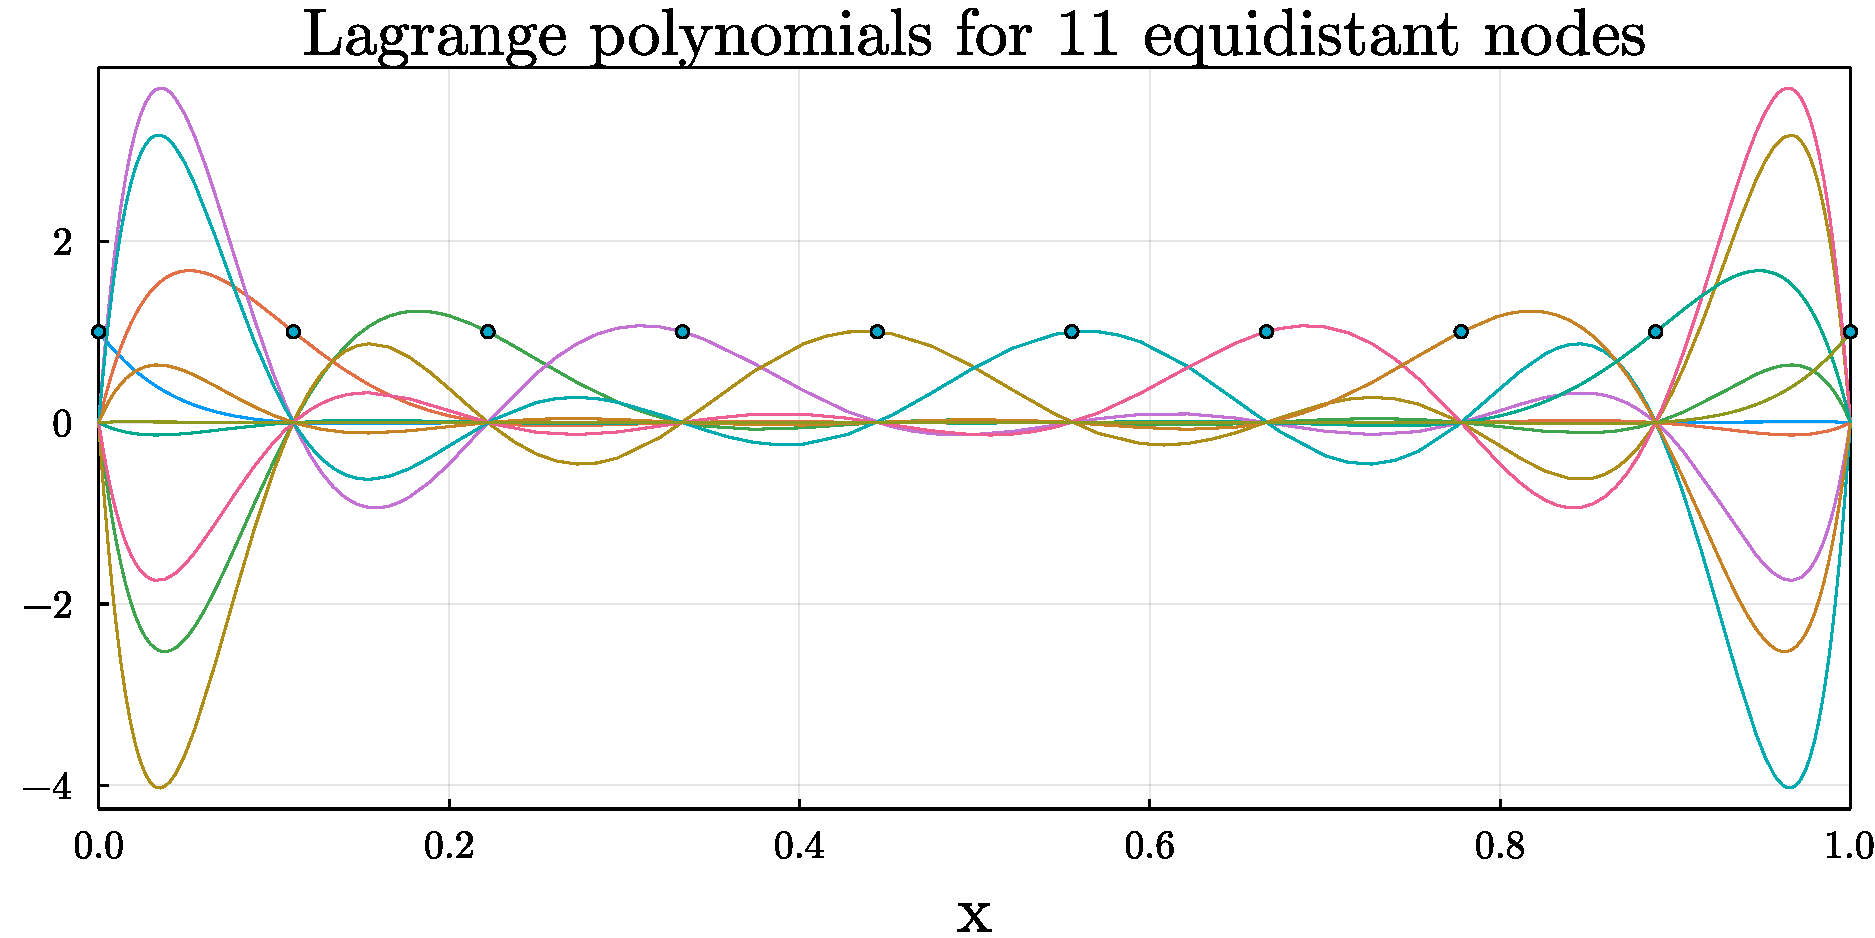
\includegraphics[width=0.8\linewidth]{figures/lagrange_10.pdf}
    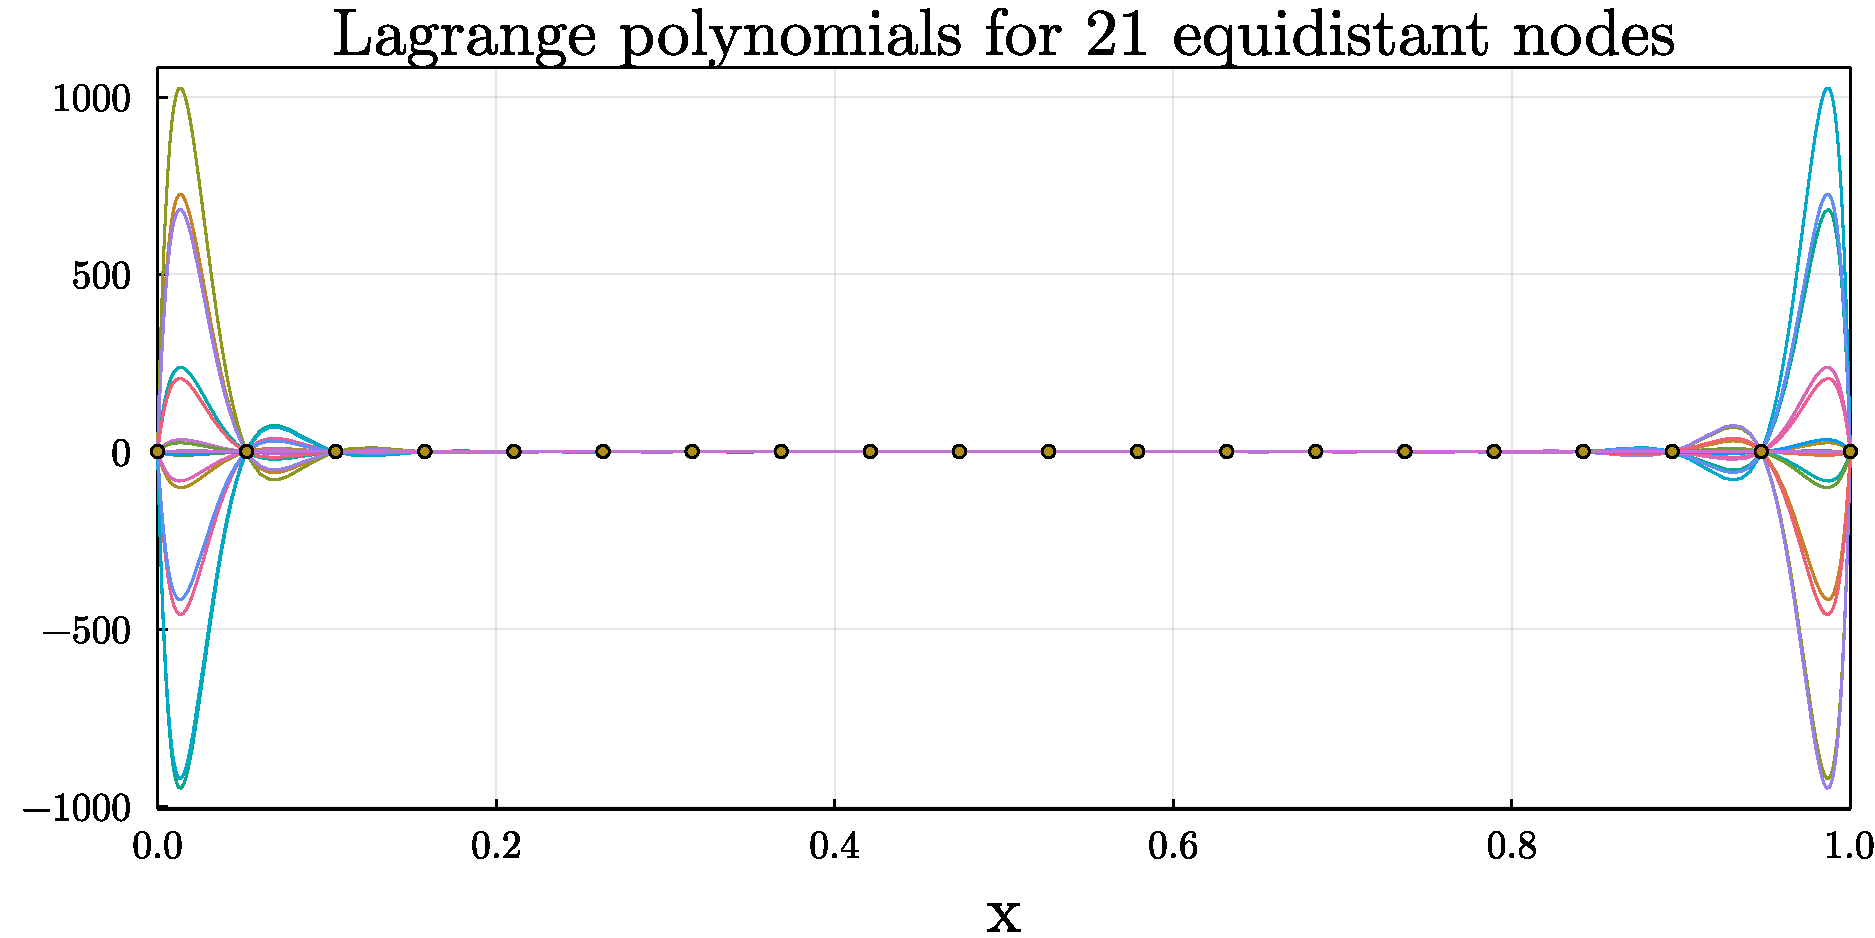
\includegraphics[width=0.8\linewidth]{figures/lagrange_20.pdf}
    \caption{Lagrange polynomials associated with equidistant nodes over the $(0, 1)$ interval.}%
    \label{fig:lagrange}
\end{figure}

\subsection{Gregory--Newton interpolation}
By Taylor's formula,
any polynomial~$p$ of degree $n$ may be expressed as
\begin{equation}
    \label{eq:taylor}
    p(x) = p(0) + p'(0) x + \frac{p''(0)}{2} x^2 + \dotsc + \frac{p^{(n)}(0)}{n!} x^n.
\end{equation}
In other words, the constant coefficient can be obtained by evaluating the polynomial at 0,
the linear coefficient can be identified by evaluating the first derivative at 0,
and so on.
Assume now that we are given the values taken by~$p$ when evaluated at the integer numbers $\{0, \dotsc, n\}$,
which we denote by $p_0, \dotsc, p_n$.
We ask the following question:
can we find a formula similar in spirit to~\eqref{eq:taylor},
but including only evaluations of $p$ and not of its derivatives?
To answer this question, we introduce the difference operator $\Delta$ which acts on functions as follows:
\[
    \Delta f(x) = f(x+1) - f(x).
    % (p_0, p_1, \dotsc) \mapsto (p_1 - p_0, p_2 - p_1, \dotsc).
\]
The operator~$\Delta$ is a linear operator on the space of continuous functions.
It maps constant functions to 0,
and the linear function~$x$ to the constant function~$1$,
suggesting a resemblance with the differentiation operator.
In order to further understand this connection,
let us define the \emph{falling power} of a real number $x$ as
\[
    x^{\underline{k}} = x (x-1) (x-2) \dots (x-k+1).
\]
We then have that
\begin{align*}
    \Delta x^{\underline{k}}
    &= (x+1) x (x-1) \dots (x-k+2) - x (x-1) (x-2) \dots (x-k+1) \\
    &= \bigl((x+1) - (x-k+1)\bigr) \bigl(x (x-1) \dots (x-k+2)\bigr) = k x^{\underline{k-1}}
\end{align*}
In other words,
the action of the difference operator on falling powers mirrors that of the differentiation operator on monomials.
The falling powers form a basis of the space of polynomials,
and so any polynomial in~$\poly(n)$, i.e.\ of degree less than or equal to $n$, can be expressed as
\begin{equation}
    \label{eq:gregory_newton}
    p(x) = \alpha_0 + \alpha_1 x^{\underline{1}} + \alpha_2 x^{\underline{2}} + \dotsb + \alpha_n x^{\underline{n}}.
\end{equation}
It is immediate to show that $\alpha_i = \Delta^i p(0)$,
where $\Delta^i p$ denotes the function obtained after~$i$ applications of the operator~$\Delta$.
Therefore, any polynomial of degree less than or equal to~$n$ may be expressed as
\begin{equation}
    \label{eq:gregory_newton_actually}
    p(x) = p(0) + \Delta p(0) x^{\underline{1}} + \frac{\Delta^2}{2} x^{\underline{2}} + \dotsb + \frac{\Delta^n p(0)}{n!} x^{\underline{n}}.
\end{equation}
An expansion of the form~\eqref{eq:gregory_newton_actually} is called a \emph{Newton series},
which is the discrete analog of the continuous Taylor series.
From the definition of~$\Delta$,
it is clear that the coefficients in~\eqref{eq:gregory_newton_actually} depend only on~$p(0), \dotsc, p(n)$.
We conclude that, given points $n+1$ points $(i, p_i)$ for $i \in \{0, \dotsc, n\}$,
the unique interpolating polynomial can be obtained from~\eqref{eq:gregory_newton_actually}.

\begin{example}
    \label{example:gregory_newton}
    Let us use~\eqref{eq:gregory_newton} in order to calculate the value of
    \[
        S(n) := \sum_{i=0}^{n} i^2.
    \]
    Since $\Delta S(n) = (n+1)^2$,
    which is a second degree polynomial in $n$,
    we deduce that $S(n)$ is a polynomial of degree 3.
    % Notice the slight abuse of notation here:
    % since $S(n)$ is well-defined only for $n \in \nat$,
    % $\Delta S(n)$ is also well-defined
    Let us now determine its coefficients.
    \begin{center}
    \begin{tabular}{|c|c|c|c|c|}
        \hline
        $n$    & $0$ & $1$ & $2$ & $3$ \\ \hline
        $\Delta^0 S(n)$ & $\mathbf{0}$ & $1$ & $5$ & $14$ \\ \hline
        $\Delta^1 S(n)$ & $\mathbf{1}$ & $4$ & $9$ &  \\ \hline
        $\Delta^2 S(n)$ & $\mathbf{3}$ & $5$ & & \\ \hline
        $\Delta^3 S(n)$ & $\mathbf{2}$ & & & \\ \hline
    \end{tabular}
    \end{center}
    We conclude that
    \[
        S(n) = \mathbf{1} n + \frac{\mathbf{3}}{2!} n(n-1) + \frac{\mathbf{2}}{3!} n(n-1)(n-2)
        = \frac{n (2n+1) (n+1)}{6}
    \]
\end{example}
Notice that when falling powers are employed as polynomial basis,
the matrix in~\eqref{eq:linear_system_interpolation} is lower triangular,
and the algorithm described in~\cref{example:gregory_newton} could be replaced by the forward substitution method.
Whereas the coefficients of the Lagrange interpolant can be obtained immediately from the values of~$u$ at the nodes,
calculating the coefficients of the expansion in~\eqref{eq:gregory_newton} requires $\mathcal O(n^2)$ operations.
However, this method has several advantages over Lagrange interpolation:
\begin{itemize}
    \item
        If a point~$(n+1, p_{n+1})$ is added to the set of interpolation points,
        only one additional term, corresponding to the falling power~$x^{\underline{n+1}}$,
        has to be calculated in~\eqref{eq:gregory_newton_actually}.
        All the other coefficients are unchanged.
        Therefore, the Gregory--Newton approach is well-suited for incremental interpolation.

    \item
        The Gregory--Newton interpolation method method is more numerically stable than Lagrange interpolation,
        because none of the basis functions take very large values.

    \item
        A polynomial in the form of a Newton series can be evaluated efficiently using Horner's method,
        which is based on rewriting the polynomial as
        \[
            p(x) = \alpha_0 + x \biggl( \alpha_1 + (x-1)  \Bigl( \alpha_2 + (x-2)\bigl(\alpha_3 + (x-3) \dotsc \bigr) \Bigr)  \biggr).
        \]
        Evaluating this expression starting from the innermost bracket leads to an algorithm with a cost scaling linearly with the degree of the polynomial.
\end{itemize}

\subsubsection*{Non-equidistant nodes}%
So far,
we have described the Gregory--Newton method in the simple setting where interpolation nodes are just a sequence of successive natural numbers.
The method can be generalized to the setting of nodes $x_0 \neq \dotsc \neq x_n$ which are not necessarily equidistant.
In this case, we take as basis the following functions instead of the falling powers:
\begin{equation}
    \label{eq:basis_newton}
    \varphi_{i}(x) = (x - x_0) (x - x_1) \dotsc (x - x_{i-1}),
\end{equation}
with the convention that the empty product is 1.
By~\eqref{eq:linear_system_interpolation},
the coefficients of the interpolating polynomial in this basis solve the following linear system:
\begin{equation}
    \label{eq:matrix_newton}
    \begin{pmatrix}
        1 &         & \ldots &        & 0  \\
        1 & x_1-x_0 &        &        &    \\
        1 & x_2-x_0 & (x_2-x_0)(x_2-x_1) &        & \vdots   \\
        \vdots & \vdots  &        & \ddots &    \\
        1 & x_n-x_0 & \ldots & \ldots & \prod_{j=0}^{n-1}(x_n - x_j)
    \end{pmatrix}
    \begin{pmatrix}
        \alpha_0 \\
        \alpha_1 \\
        \alpha_2 \\
        \vdots \\
        \alpha_n
    \end{pmatrix}
    =
    \begin{pmatrix}
        u_0 \\
        u_1 \\
        u_2 \\
        \vdots \\
        u_n
    \end{pmatrix}.
\end{equation}
This system could be solved using, for example, forward substitution.
Clearly $\alpha_0 = u_0$,
and then from the second equation we obtain
\[
    \alpha_1 = \frac{u_1 - u_0}{x_1 - x_0} =: [u_0, u_1],
\]
which may be viewed as an approximation of the slope of~$u$ at $x_0$.
The right-hand side of this equation is an example of a \emph{divided difference}.
In general, divided differences are defined recursively as follows:
\[
    [u_{0}, u_{2}, \dotsc, u_{d}] := \frac{[u_{1}, \dotsc, u_{d}] - [u_{0}, \dotsc, u_{d-1}]}{x_{d}-x_{0}}, \qquad [u_i] = u_i.
\]
It is possible to find an expression for the coefficients of the interpolating polynomials in terms of these divided differences.
\begin{proposition}
    Assume that $(x_0, u_0), \dotsc, (x_n, u_n)$ are $n+1$ points in the plane with distinct abcissae.
    Then the interpolating polynomial of degree $n$ may be expressed as
    \[
        p(x) = \sum_{i=0}^{n} [u_0, \dotsc, u_n] \varphi_i(x),
    \]
    where $\varphi_i(x)$, for $i = 0, \dotsc, n$, are the basis functions defined in~\eqref{eq:basis_newton}.
\end{proposition}
\begin{proof}
    The statement is true for $n = 0$.
    Reasoning by induction, we assume that it holds true for polynomials of degree up to $n-1$.
    Let $p_1(x)$ and $p_2(x)$ be the interpolating polynomials at the points
    $x_0, x_1, \dotsc, x_{n-2}, x_{n-1}$ and $x_0, x_1, \dotsc, x_{n-2}, x_{n}$, respectively.
    Then
    \begin{equation}
        \label{eq:interpolating_polynomial}
        p(x) = p_1(x) + \frac{x - x_{n-1}}{x_n - x_{n-1}} \bigl(p_2(x) - p_1(x)\bigr)
    \end{equation}
    is a polynomial of degree~$n$ that interpolates all the data points.
    By the induction hypothesis,
    it holds that
    \begin{align*}
        p_1(x) &= u_0 + [u_0, u_1] (x - x_0) + \dotsc + [u_0, u_1, \dotsc, u_{n-2}, \mathbf{u_{n-1}}] \prod_{i=0}^{n-2} (x - x_i), \\
        p_2(x) &= u_0 + [u_0, u_1] (x - x_0) + \dotsc + [u_0, u_1, \dotsc, u_{n-2}, \mathbf{u_{n}}] \prod_{i=0}^{n-2} (x - x_i).
    \end{align*}
    Here we used bold font to emphasize the difference between the two expressions.
    Substituting these expressions in~\eqref{eq:interpolating_polynomial},
    we obtain
    \begin{align*}
        p(x) =
        &u_0 + [u_0, u_1] (x - x_0) + \dotsc + [u_0, \dotsc, u_{n-2}] \prod_{i=0}^{n-2} (x - x_i)  \\
        & + \frac{[u_0, u_1, \dotsc, u_{n-2}, u_{n-1}] - [u_0, u_1, \dotsc, u_{n-2}, u_{n}]}{x_n - x_{n-1}} \prod_{i=0}^{n-1} (x - x_i).
    \end{align*}
    In \cref{exercise:divided_differences},
    we show that divided differences are invariant under permutations of the data points,
    and so we have that
    \[
        \frac{[u_0, u_1, \dotsc, u_{n-2}, u_{n-1}] - [u_0, u_1, \dotsc, u_{n-2}, u_{n}]}{x_n - x_{n-1}} = [u_0, \dotsc, u_n],
    \]
    which enables to conclude.
    % Observing that $p(x) - u_0$ has a root at $x_0$,
    % we deduce that
    % \begin{equation}
    %     \label{eq:equation_newton}
    %     q(x) :=
    %     \frac{p(x) - u_0}{x - x_0}
    % \end{equation}
    % is a polynomial of degree at most $n-1$ that interpolates the points
    % \begin{equation}
    %     \label{eq:newton_interpolation_vi}
    %     \left(x_i, v_i\right) := \left(x_i, \frac{u_i - u_0}{x_i - x_0}\right), \qquad i = 1, \dotsc, n.
    % \end{equation}
    % Using the induction hypothesis,
    % we deduce that $q(x)$ is given by
    % \[
    %     q(x) = \sum_{i=1}^{n} [v_1, \dotsc, v_i] (x-x_1) \dotsc (x - x_{i-1})
    % \]
    % By~\cref{exercise:divided_differences},
    % it holds that
    % \[
    %     [v_1, \dotsc, v_n] = \sum_{j=1}^{n} \frac{v_{j}}{\prod_{ k \in \{1, \dotsc, n\} \backslash \{ j\}} (x_{j} - x_{k})}.
    % \]
    % Therefore, employing the expression of~$v_j$ given in~\eqref{eq:newton_interpolation_vi},
    % we have
    % \begin{align*}
    %     [v_1, \dotsc, v_n]
    %     &= \sum_{j=1}^{n} \frac{\frac{u_{j}-u_0}{x_j - x_0}}{\prod_{ k \in \{1, \dotsc, n\} \backslash \{ j\}} (x_{j} - x_{k})}
    %     = \sum_{j=1}^{n} \frac{u_{j}-u_0}{\prod_{ k \in \{0, \dotsc, n\} \backslash \{ j\}} (x_{j} - x_{k})} \\
    %     &= \sum_{j=0}^{n} \frac{u_{j}-u_0}{\prod_{ k \in \{0, \dotsc, n\} \backslash \{ j\}} (x_{j} - x_{k})} = [w_0, \dotsc, w_n],
    % \end{align*}
    % where we introduced $w_i = u_i - u_0$, for $i = 0, \dotsc, n$.
    % Now, since only differences appear in the divided difference $[w_0, \dotsc, w_n]$ and $w_i - w_j = u_i - u_j$ for all pairs $(i, j) \in \{0, \dotsc n\}^2$,
    % it is clear that
    % \[
    %     [w_0, \dotsc, w_n] = [u_0, \dotsc, u_n].
    % \]
    % Going back to~\eqref{eq:equation_newton} and rearranging,
    % we conclude that
    % \[
    %     p(x) = u_0 + (x-x_0) \left( \sum_{i=1}^{n} [u_0, \dotsc, u_n] (x-x_1) \dotsc (x - x_{i-1}) \right)
    %     =  \sum_{i=0}^{n} [u_0, \dotsc, u_{i}] \prod_{j=0}^{i-1} (x-x_j),
    % \]
    % which was the statement.
\end{proof}
\begin{example}
    Assume that we are looking for the third degree polynomial going through the points
    \[
        (-1, 10), \qquad (0, 4), \qquad (2, -2), \qquad (4, -40).
    \]
    We have to calculate $\alpha_i = [u_0, \dotsc, u_i]$ for $i \in \{0, 1, 2, 3\}$.
    It is convenient to use a table in order to calculate the divided differences:
    \begin{center}
    \begin{tabular}{|c|c|c|c|c|}
        \hline
        $i$ & $0$ & $1$ & $2$ & $3$ \\ \hline
        $[u_i]$ & $\mathbf{10}$ & $4$ & $-2$ & $-40$ \\ \hline
        $x_{i+1} - x_{i}$ & $1$ & $2$ & $2$ &  \\ \hline
        $[u_i, u_{i+1}]$ & $\mathbf{-6}$ & $-3$ & $-19$ &  \\ \hline
        $x_{i+2} - x_{i}$ & $3$ & $4$ &  &  \\ \hline
        $[u_i, u_{i+1}, u_{i+2}]$ & $\mathbf{1}$ & $-4$ & & \\ \hline
        $x_{i+3} - x_{i}$ & $5$  & &  &  \\ \hline
        $[u_i, u_{i+1}, u_{i+2}, u_{i+3}]$ & $\mathbf{-1}$ & & & \\ \hline
    \end{tabular}
    \end{center}
    We deduce that the expression of the interpolating polynomial is
    \[
        p(x)
        = \mathbf{10} + (\mathbf{-6})(x+1) + \mathbf{1} (x+1)x + (\mathbf{-1}) (x+1)x(x-2)
        = - x^3 + 2 x^2 + -3x + 4.
    \]
\end{example}

\subsection{Interpolation error}
Assume that~$u(x)$ is a continuous function and denote by $\widehat u(x)$ its interpolation through the points~$(x_i, u_i)$,
for $i = 0, \dotsc, n$.
In this section, we study the behavior of the error in the limit as $n \to \infty$.

\begin{theorem}
    [Interpolation error]
    \label{theorem:interpolation_error}
    Assume that~$u\colon [a, b] \to \real$ is a function in $C^{n+1}([a, b])$ and let~$x_0, \dotsc, x_n$ denote $n+1$ distinct interpolation nodes.
    Then for all $x \in [a, b]$,
    there exists~$\xi = \xi(x)$ in the interval $[a, b]$ such that
    \[
        e_n(x) := u(x) - \widehat u(x) = \frac{u^{(n+1)}(\xi)}{n+1!} (x-x_0) \dotsc (x - x_n).
    \]
\end{theorem}
\begin{proof}
    The statement is obvious if $x \in \{x_0, \dotsc, x_n\}$,
    so we assume from now on that $x$ does not coincide with an interpolation node.
    Let us use the compact notation $\omega_n = \prod_{i=0}^n (x - x_i)$ and introduce the function
    \begin{equation}
        \label{eq:interpolation_error}
        g(t) = e_n(t) \omega_n(x) - e_n(x) \omega_n(t).
    \end{equation}
    The function $g$ is smooth and takes the value~0 when evaluated at~$x_0, \dotsc, x_n, x$.
    Since $g$ has $n+2$ roots in the interval $[a, b]$,
    Rolle's theorem implies that $g'$ has $n+1$ distinct roots in~$(a, b)$.
    Another application of Rolle's theorem yields that $g''$ has $n$ distinct roots in~$(a, b)$.
    Iterating this reasoning, we deduce that $g^{(n+1)}$ has one root~$t_*$ in $(a, b)$.
    From~\eqref{eq:interpolation_error},
    we calculate that
    \begin{equation}
        \label{eq:interpolation_error_proof}
        g^{(n+1)}(t) = e_n^{(n+1)}(t) \omega_n(x) - e_n(x) \omega_n^{(n+1)}(t)
        = u^{(n+1)}(t) \omega_n(x) - e_n(x) (n+1)!.
    \end{equation}
    Here we employed the fact that $\widehat u^{(n+1)}(t) = 0$,
    because $\widehat u$ is a polynomial of degree at most $n$.
    Evaluating~\eqref{eq:interpolation_error_proof} at~$t_*$ and rearranging,
    we obtain that
    \[
        e_n(x) = \frac{u^{(n+1)}(t_*)}{(n+1)!} \omega_n(x),
    \]
    which completes the proof.
\end{proof}
As a corollary to~\cref{theorem:interpolation_error},
we deduce the following error bound.
\begin{corollary}
    [Upper bound on the interpolation error]
    \label{corollary:interpolation_error}
    Assume that $u$ is smooth in $[a, b]$ and that
    \[
        \sup_{x \in [a, b]} \abs{u^{(n+1)}(x)} \leq C_{n+1}.
    \]
    Then
    \begin{equation}
        \label{eq:upper_bound_interp_error}
        \forall x \in [a, b], \qquad
        \abs{e_n(x)} \leq \frac{C_{n+1}}{n+1} h^{n+1}
    \end{equation}
    where $h$ is the maximum spacing between two successive interpolation nodes.
\end{corollary}
\begin{proof}
By~\cref{theorem:interpolation_error},
we have
\begin{equation}
    \label{eq:bound_error_from_theorem}
    \forall x \in [a, b], \qquad
    \abs{e_n(x)} \leq \frac{C_{n+1}}{(n+1)!} \abs[Big]{(x-x_0) \dotsc (x-x_n)}.
\end{equation}
The product on the right-hand side is bounded from above by
\begin{equation}
    \label{eq:interpolation_bound_product}
    \frac{h^2}{4} \times 2h \times 3h \times 4h \times \dotsb \times nh = \frac{n! h^{n+1}}{4}.
\end{equation}
The first factor comes from the fact that, if $x \in [x_i, x_{i+1}]$,
then
\[
    \abs{(x - x_i)(x - x_{i+1})} \leq \frac{(x_{i+1} - x_i)^2}{4},
\]
because the left-hand side is maximized when $x$ is the midpoint of the interval~$[x_i, x_{i+1}]$.
Substituting~\eqref{eq:interpolation_bound_product} into~\eqref{eq:bound_error_from_theorem},
we deduce the statement.
\end{proof}
Let us now introduce the supremum norm of the error over the interval $[a, b]$:
\[
    E_n = \sup_{x \in [a, b]} \abs{e_n(x)}.
\]
We ask the following natural question:
does $E_n$ tend to zero as the maximum spacing between successive nodes tends to 0?
By~\cref{corollary:interpolation_error},
the answer to this question is positive when $C_{n}$ does not grow too quickly as $n \to \infty$.
For example, as illustrated in \cref{fig:interpolation_sine},
the interpolation error for the function $u(x) = \sin(x)$,
when using equidistant interpolation nodes,
decreases very quickly as $n \to \infty$.
\begin{figure}[ht!]
    \centering
    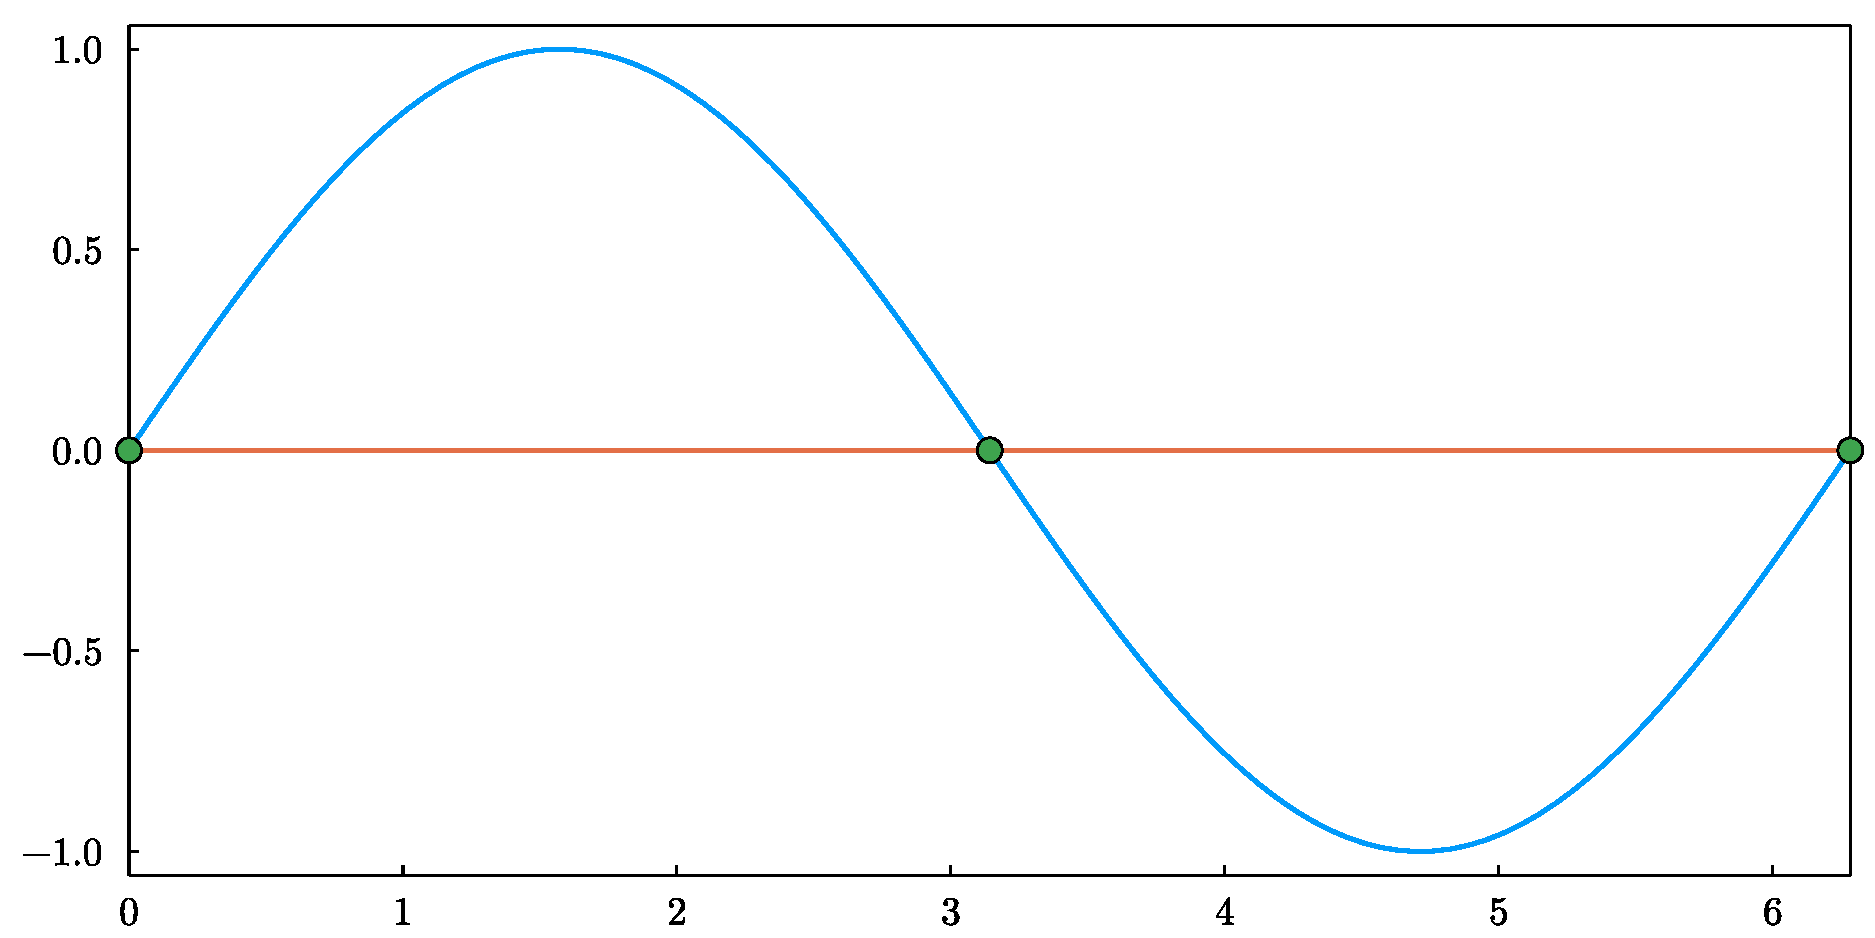
\includegraphics[width=0.49\linewidth]{figures/interpolation_sine_3.pdf}
    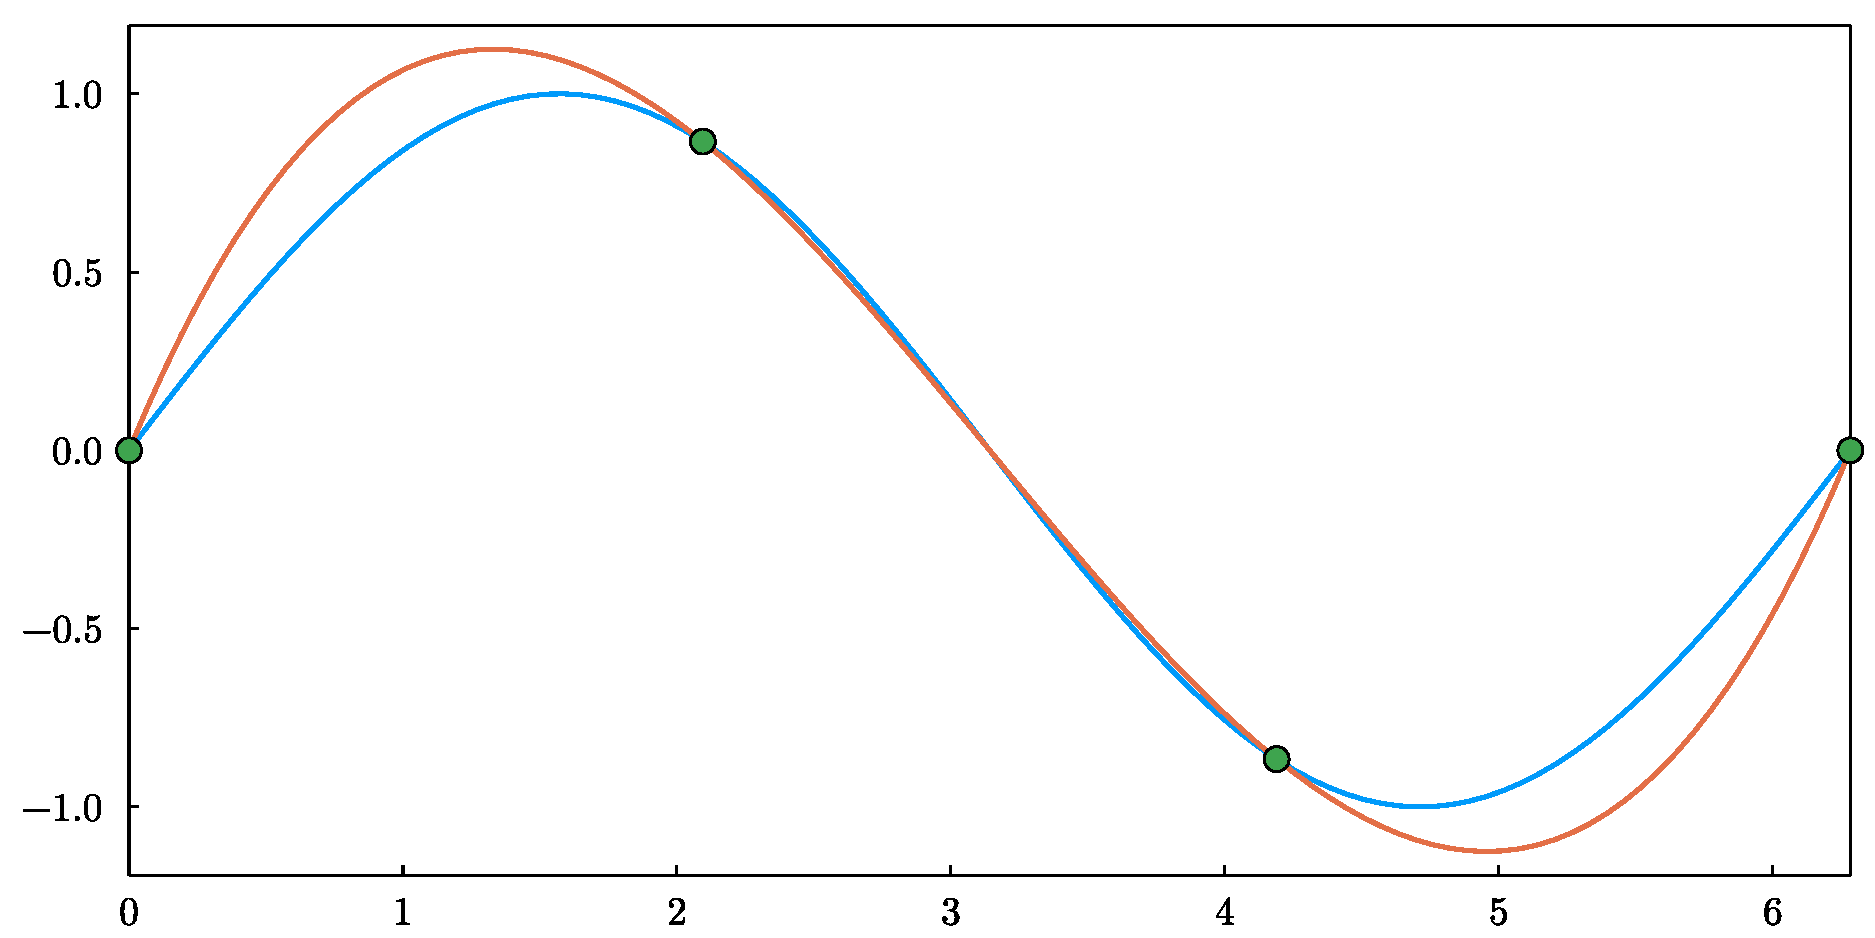
\includegraphics[width=0.49\linewidth]{figures/interpolation_sine_4.pdf}
    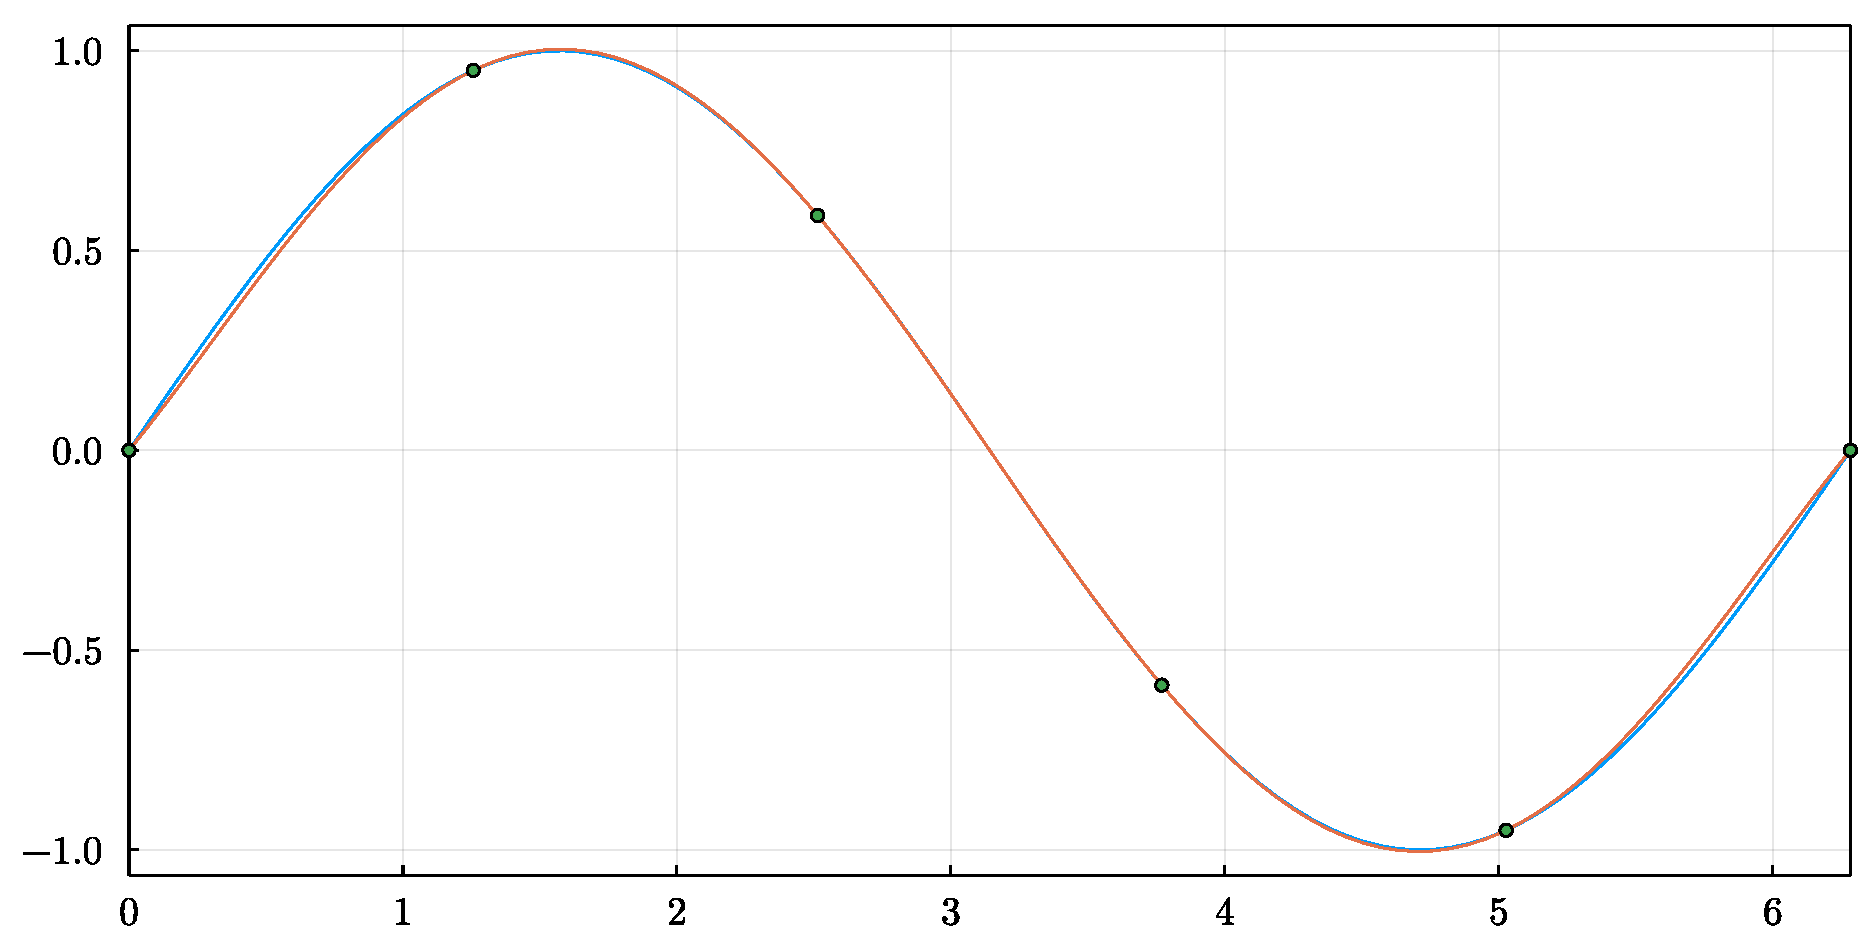
\includegraphics[width=0.49\linewidth]{figures/interpolation_sine_6.pdf}
    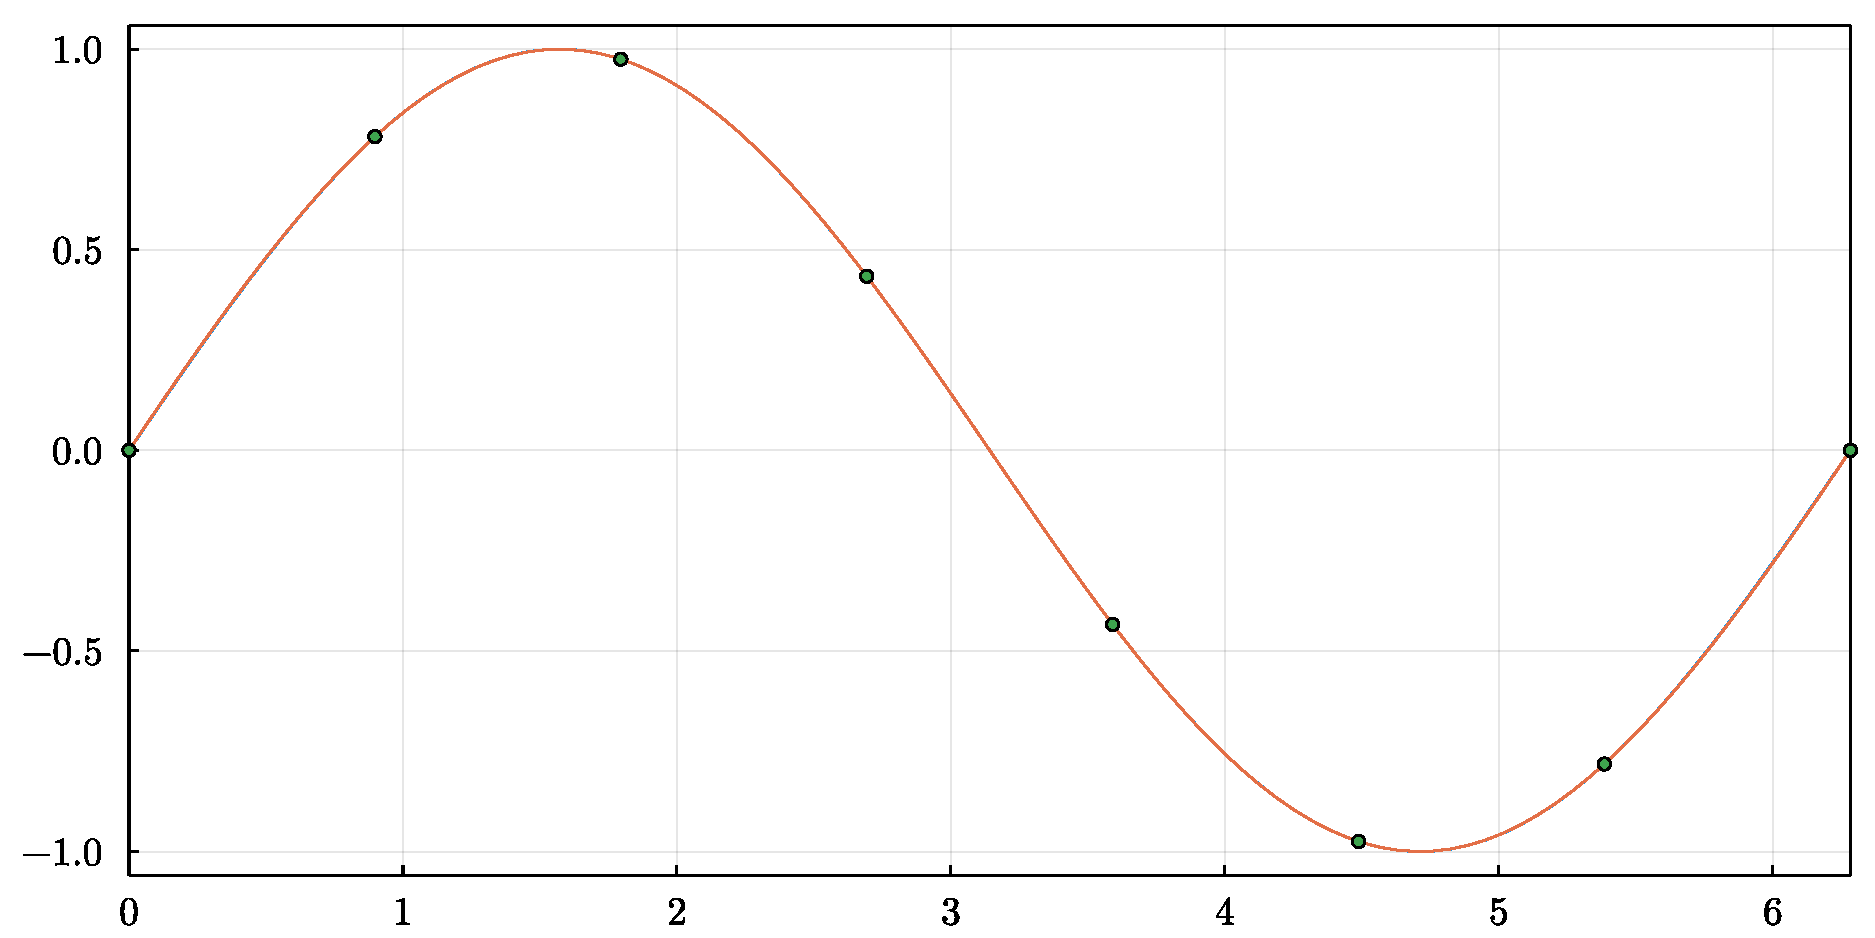
\includegraphics[width=0.49\linewidth]{figures/interpolation_sine_8.pdf}
    \caption{Interpolation (in orange) of the function $u(x) = \sin(x)$ (in blue) using 3, 4, 6, and 8 equidistant nodes.}%
    \label{fig:interpolation_sine}
\end{figure}

In some cases, however,
the constant $C_n$ grows quickly with $n$,
to the extent that $E_n$ may increase with $n$;
in this case, the maximum interpolation error grows as we add nodes!
The classic example,
in order to illustrate this potential issue,
is that of the Runge function:
\begin{equation}
    \label{eq:runge_function}
    u(x) = \frac{1}{1 + 25 x^2}.
\end{equation}
It is possible to show that,
for this function,
the upper bound in~\cref{corollary:interpolation_error} tends to $\infty$ in the limit as the number of interpolation nodes increases.
We emphasize that this does not prove that $E_n \to \infty$,
because~\eqref{eq:upper_bound_interp_error} provides only an upper bound on the error.
In fact, the interpolation error can either grow or decrease,
depending on the choice of interpolation nodes.
With equidistant nodes, it turns out that $E_n \to \infty$,
as illustrated in~\cref{fig:interpolation_runge_function}.
\begin{figure}[ht!]
    \centering
    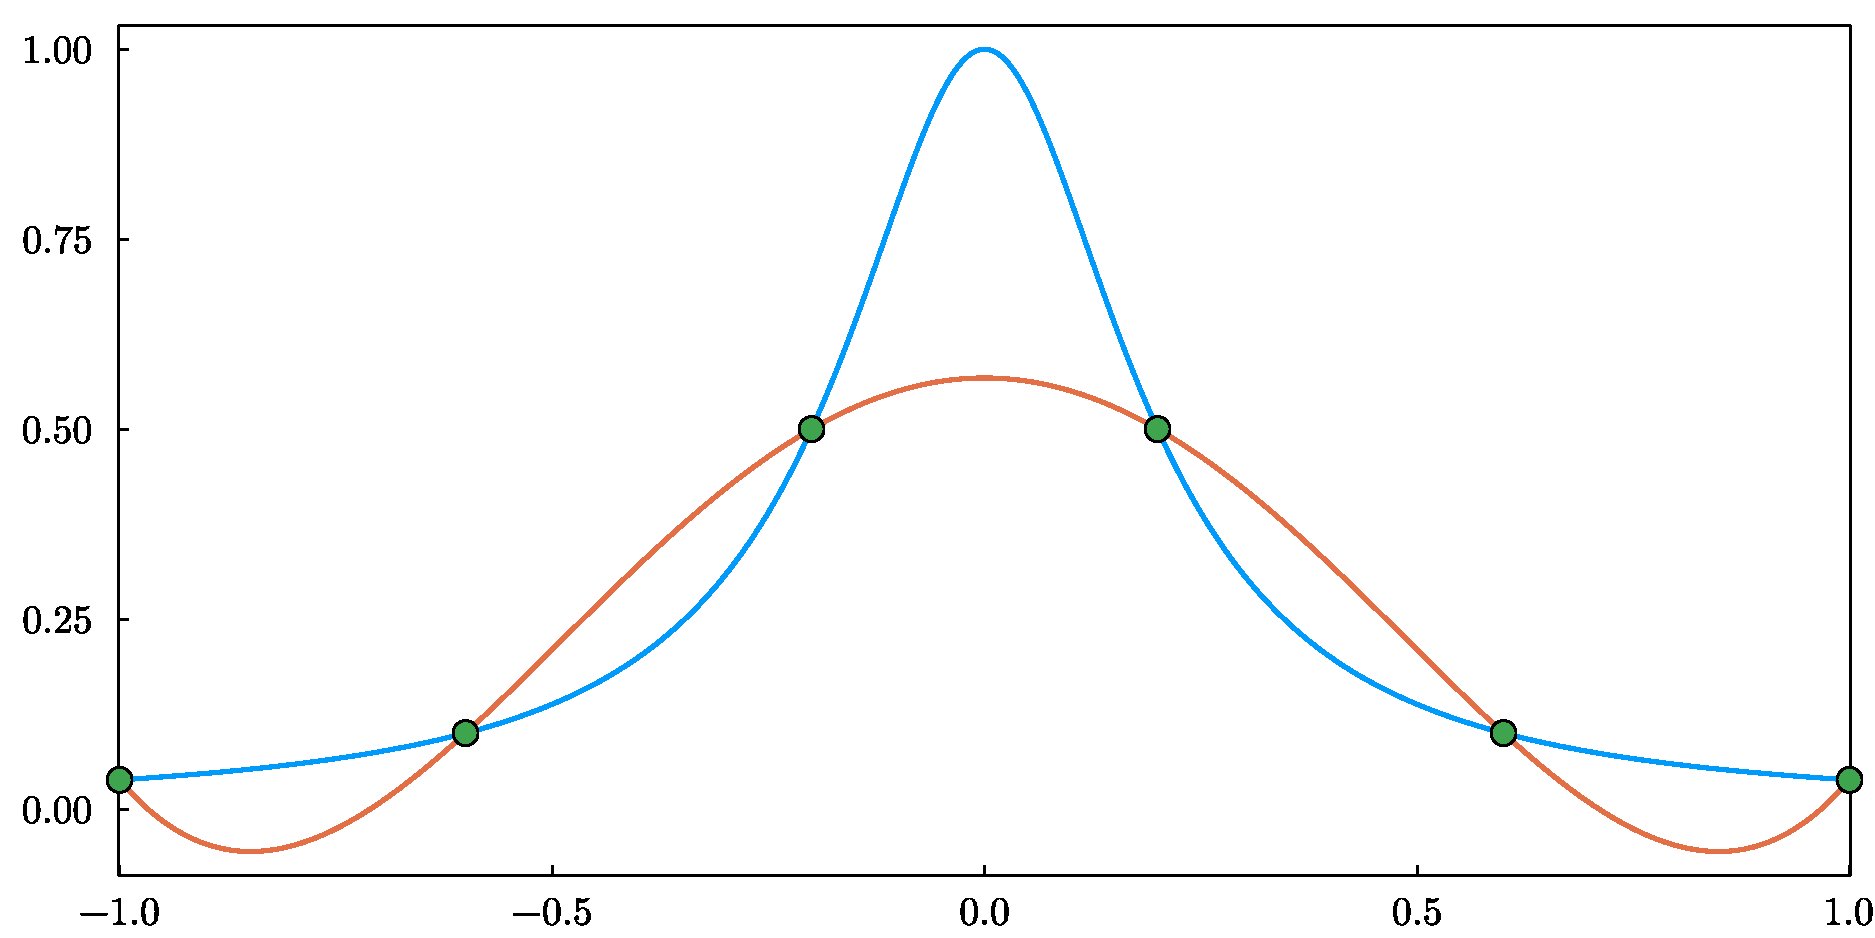
\includegraphics[width=0.49\linewidth]{figures/interpolation_runge_6.pdf}
    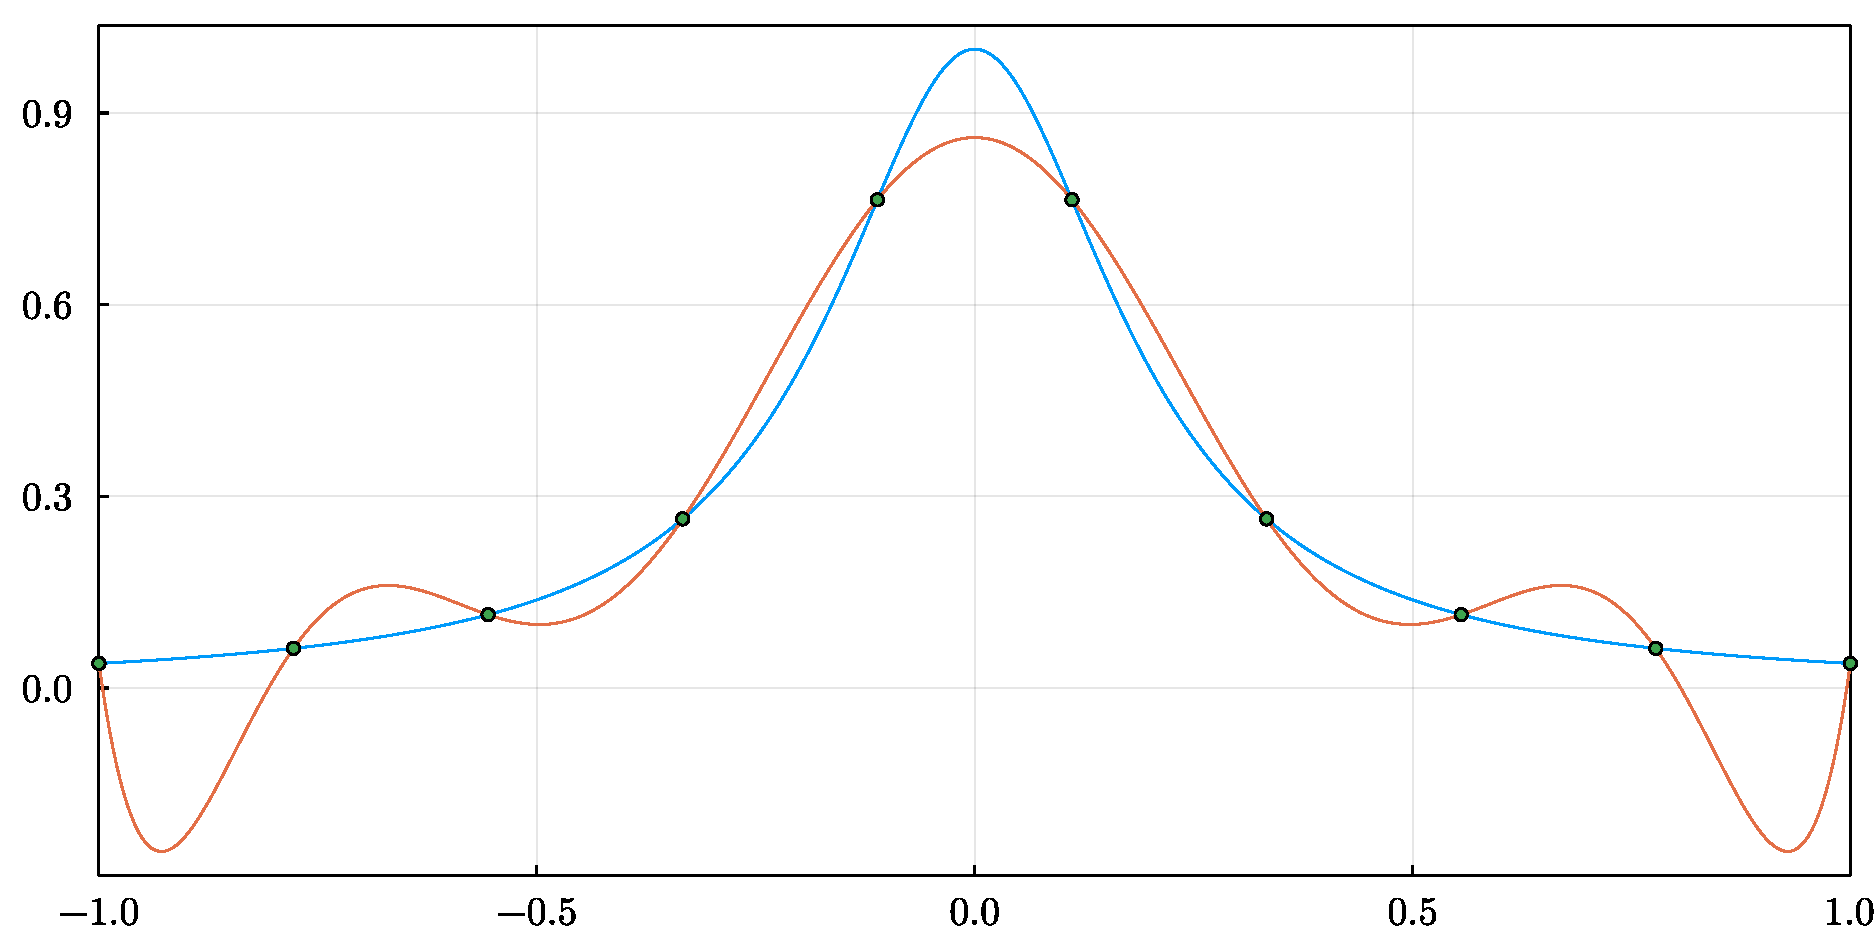
\includegraphics[width=0.49\linewidth]{figures/interpolation_runge_10.pdf}
    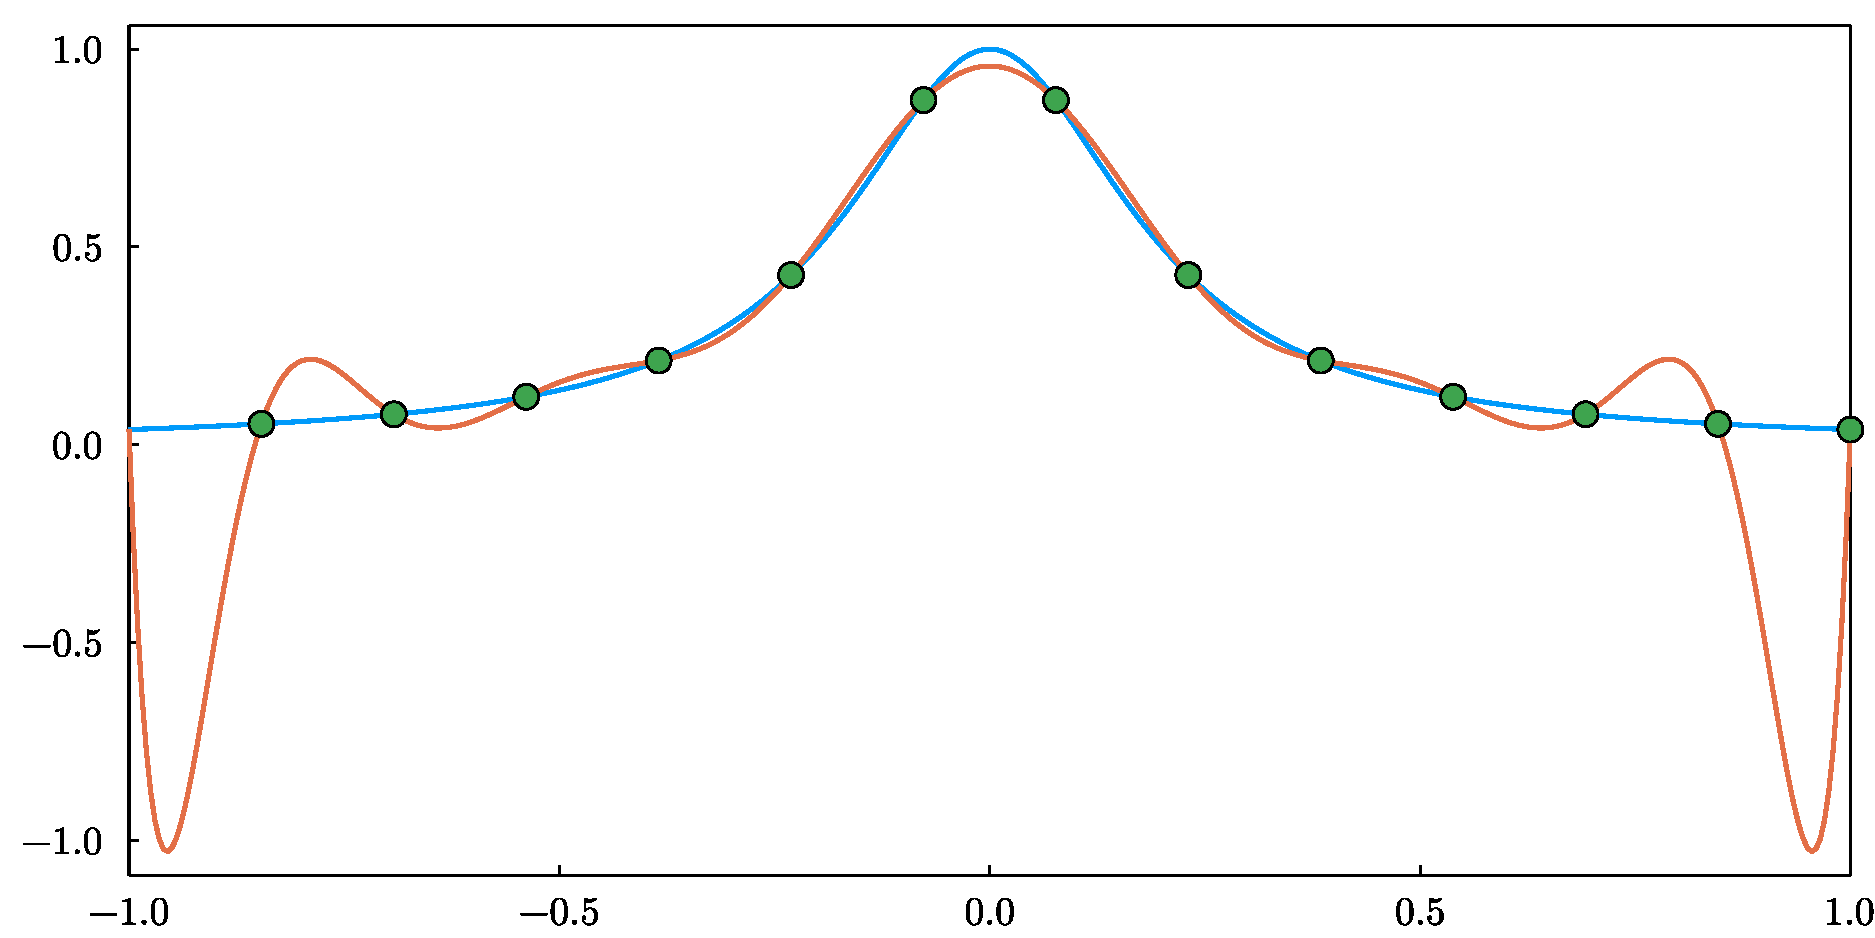
\includegraphics[width=0.49\linewidth]{figures/interpolation_runge_14.pdf}
    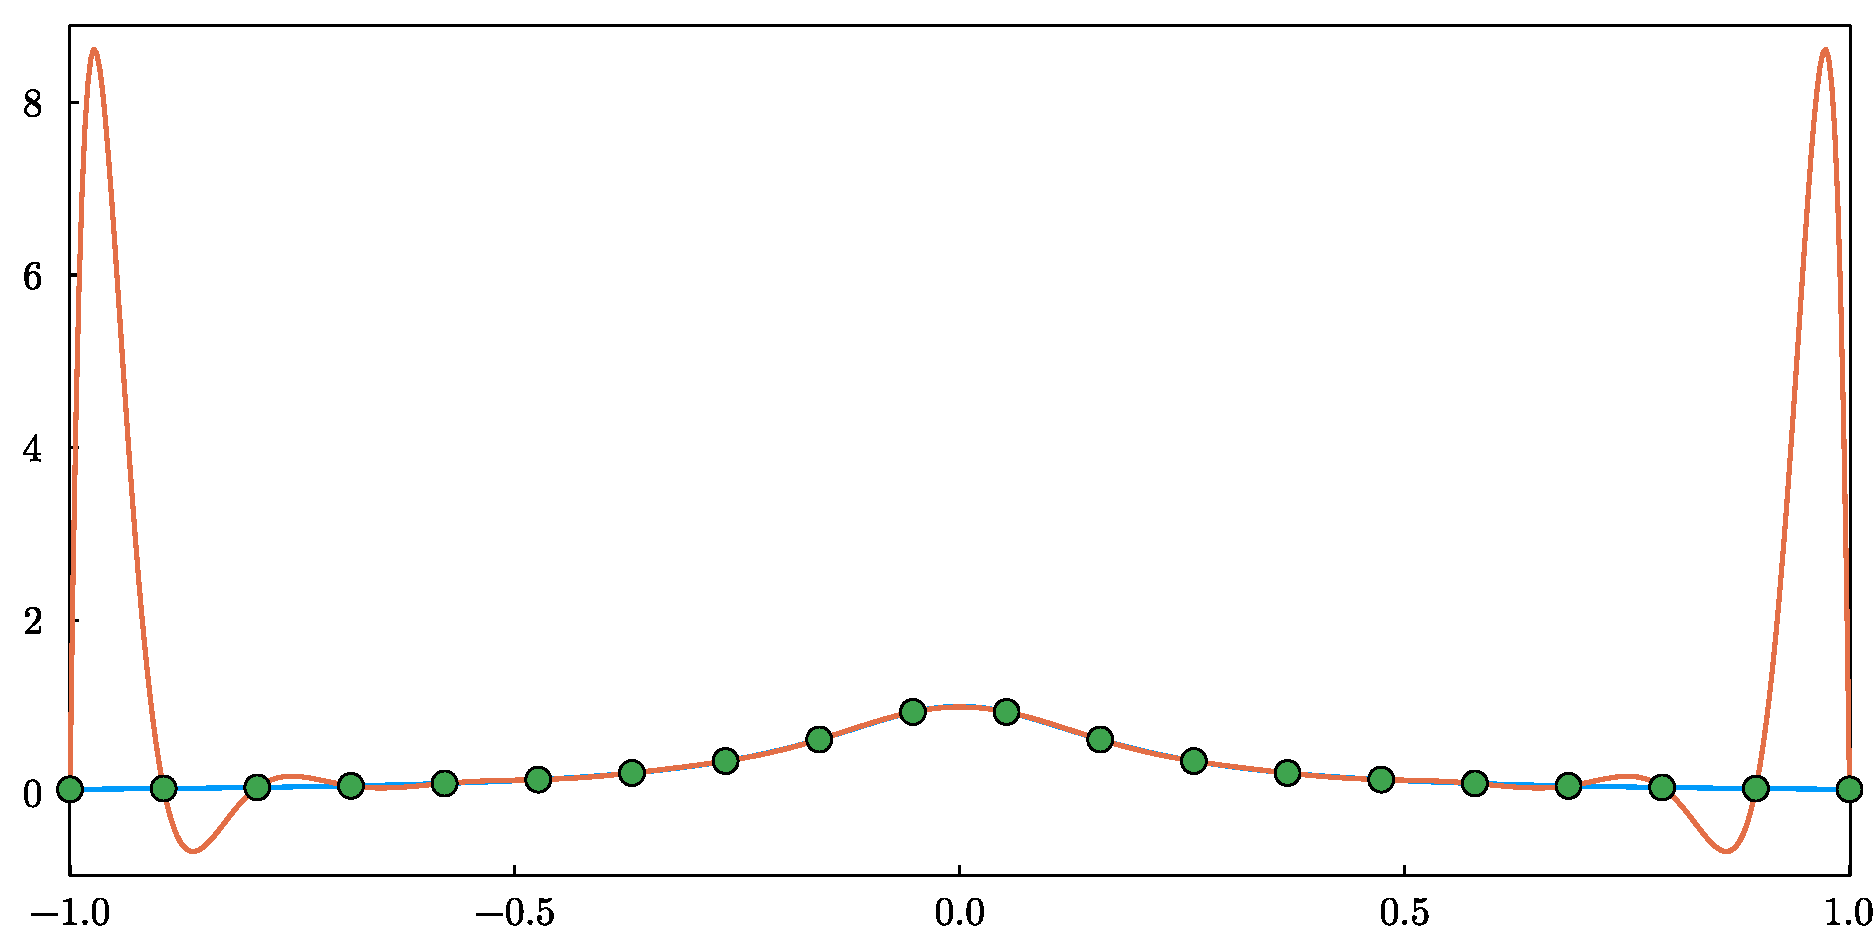
\includegraphics[width=0.49\linewidth]{figures/interpolation_runge_20.pdf}
    \caption{Interpolation (in orange) of the Runge function~\eqref{eq:runge_function} (in blue) using 6, 10, 14, and 20 equidistant nodes.}%
    \label{fig:interpolation_runge_function}
\end{figure}

\subsection{Interpolation at Chebyshev nodes}
Sometimes,
interpolation is employed as a technique for approximating functions.
The spectral collocation method, for example,
is a technique for solving partial differential equations
where a discrete solution is first calculated,
and then a continuous solution is constructed using polynomial or Fourier interpolation.
When the interpolation nodes are not given a priori as data,
it is natural to wonder whether these can be picked in such a manner that the interpolation error,
measured in the supremum norm, is minimized.
More precisely, given a continuous function~$u(x)$ and a number of nodes~$n$,
is it possible to chose nodes $x_0, \dotsc, x_n$ such that
\[
    E := \sup_{x \in [a, b]} \abs{u(x) - \widehat u(x)}
\]
is minimized?
Here $\widehat u$ is the polynomial interpolating~$u$ at the nodes.
Achieving this goal in general is a difficult task,
essentially because $\xi = \xi(x)$ is unknown in the expression of the interpolation error from~\cref{theorem:interpolation_error}:
\[
    e_n(x) = \frac{u^{(n+1)}(\xi)}{n+1!} (x-x_0) \dotsc (x - x_n).
\]
In view of this difficulty,
we will focus on the simpler problem of finding interpolation nodes
such that the product $(x-x_0) \dotsc (x - x_n)$ is minimized in the supremum norm.
This problem amounts to finding the optimal interpolation nodes,
in the sense that~$E$ is minimized,
in the particular case where $u$ is a polynomial of degree $n+1$,
because in this case $u^{n+1}(\xi)$ is a constant factor.
It turns out that this problem admits an explicit solution,
which we will deduce from the following theorem.
\begin{theorem}
    [Minimum $\infty$ norm]
    \label{theorem:minimum_infty_norm}
    Assume that $p$ is a monic polynomial of degree $n$:
    \[
        p(x) = \alpha_0 + \alpha_1 x + \dotsb + \alpha_{n-1} x^{n-1} + \mathbf{1} x^n.
    \]
    Then it holds that
    \begin{equation}
        \label{eq:chebychev_lower_bound}
        \sup_{x \in [-1, 1]} \abs{p(x)} \geq \frac{1}{2^{n-1}}.
    \end{equation}
    In addition, the lower bound is achieved for~$p(x) = 2^{-(n-1)} T_n(x)$,
    where $T_n$ is the Chebyshev polynomial of degree~$n$:
    \begin{equation}
        \label{eq:chebyshev_polynomial}
        T_n(x) = \cos(n\arccos x) \qquad (-1 \leq x \leq 1).
    \end{equation}
\end{theorem}
\begin{proof}
    By~\cref{exercise:chebychev},
    the polynomial $x \mapsto 2^{-(n-1)} T_n(x)$ is indeed monic,
    and it is clear that it achieves the lower bound~\eqref{eq:chebychev_lower_bound}
    since $\abs{T_n(x)} \leq 1$.

    In order to prove~\eqref{eq:chebychev_lower_bound},
    we assume by contradiction that there was a different monic polynomial~$\widetilde p$ of degree~$n$ such that
    \begin{equation}
        \label{eq:chebyshev_minimum}
        \sup_{x \in [-1, 1]} \abs{\widetilde p(x)} < \frac{1}{2^{n-1}}.
    \end{equation}
    Let us introduce $x_i = \cos(i \pi/n)$, for $i = 0, \dotsc, n$,
    and observe that
    \[
        p(x_i) = 2^{-(n-1)} T_n(x_i) = 2^{-(n-1)} (-1)^i.
    \]
    The function $q(x) := p(x) - \widetilde p(x)$ is a polynomial of degree at most $n-1$ which,
    by the assumption~\eqref{eq:chebyshev_minimum},
    is strictly positive at $x_0, x_2, x_4, \dotsc$ and strictly negative at $x_1, x_3, x_5, \dotsc$.
    Therefore, the polynomial $q(x)$ changes sign at least $n$ times and so,
    by the intermediate value theorem, it has at least $n$ roots.
    But this is impossible, because $q(x) \neq 0$ and $q(x)$ is of degree at most $n-1$.
\end{proof}

From~\cref{theorem:minimum_infty_norm},
we deduce the following corollary.
\begin{corollary}
    [Chebyshev nodes]
    \label{corollary:chebyshev_nodes}
    Assume that $x_0 < x_1 < \dotsc < x_n$ are in the interval $[a, b]$.
    The supremum norm of the product $(x-x_0) \dotsb (x-x_n)$ over~$[a, b]$ is minimized when
    \begin{equation}
        x_i = a + (b-a) \frac{1 + \cos \left( (2i + 1) \frac{\pi}{2 n} \right)}{2}
    \end{equation}
        % \label{eq:optimal_product}
        % (x-x_0) \dotsb (x-x_n) = \frac{(b-a)^n}{2^{2n-1}} T_n\left(\frac{a + b - 2x}{a - b}\right).
    % \end{equation}
    % In particular, if $a = -1$ and $b = 1$,
    % then the nodes $x_0, \dotsc, x_n$ must coincide with the roots of the Chebyshev polynomial of degree~$n$:
    % \[
        % x_i = \cos \left( (2i + 1) \frac{\pi}{2} \right).
    % \]
\end{corollary}
\begin{proof}
    We consider the affine change of variable
    \begin{align*}
        \zeta\colon &[-1, 1] \to [a, b]; \\
                    &y \mapsto \frac{a + b + y (b - a)}{2}.
    \end{align*}
    The function
    \begin{align*}
        p(y) &:= \frac{2^n}{(b-a)^n} \bigl(\zeta(y)-x_0\bigr) \dotsb \bigl(\zeta(y)-x_n\bigr) \\
             &= \bigl(y-y_0\bigr) \dotsb \bigl(y-y_n\bigr), \qquad y_i = \zeta^{-1}(x_i),
    \end{align*}
    is a monic polynomial of degree~$n$ such that
    \begin{equation}
        \label{eq:change_of_variable}
        \sup_{y \in [-1, 1]} \abs{p(y)} = \frac{2^n}{(b-a)^n} \sup_{x \in [a, b]} \abs{(x-x_0) \dotsc (x - x_n)}.
    \end{equation}
    By~\cref{theorem:minimum_infty_norm},
    the left-hand side is minimized when $p$ is equal to $2^{-(n-1)} T_n(y)$,
    i.e.\ when the roots of $p$ coincide with the roots of $T_n$.
    This occurs when
    \[
        y_i = \zeta^{-1}(x_i) = \cos \left( (2i + 1) \frac{\pi}{2 n} \right).
    \]
    Applying the inverse change of variable $x_i = \zeta(y_i)$,
    we deduce the result.
\end{proof}

\Cref{corollary:chebyshev_nodes} establishes a link with interpolation.
The nodes
\begin{equation}
    x_i = a + (b-a) \frac{1 + \cos \left( (2i + 1) \frac{\pi}{2 n} \right)}{2}, \qquad i = 0, \dotsc, n,
\end{equation}
are known as Chebyshev nodes and,
more often than not, employing these nodes for interpolation produces much better results than using equidistant rodes,
both in the case where~$u$ is a polynomial of degree $n+1$,
as we just proved,
but also for general~$u$.
As an example we plot in \cref{fig:cheb_runge} the interpolation of the Runge function using Chebyshev nodes.
In this case, the interpolating polynomial converges uniformly to the Runge function as we increase the number of interpolation nodes!
\begin{figure}[ht]
    \centering
    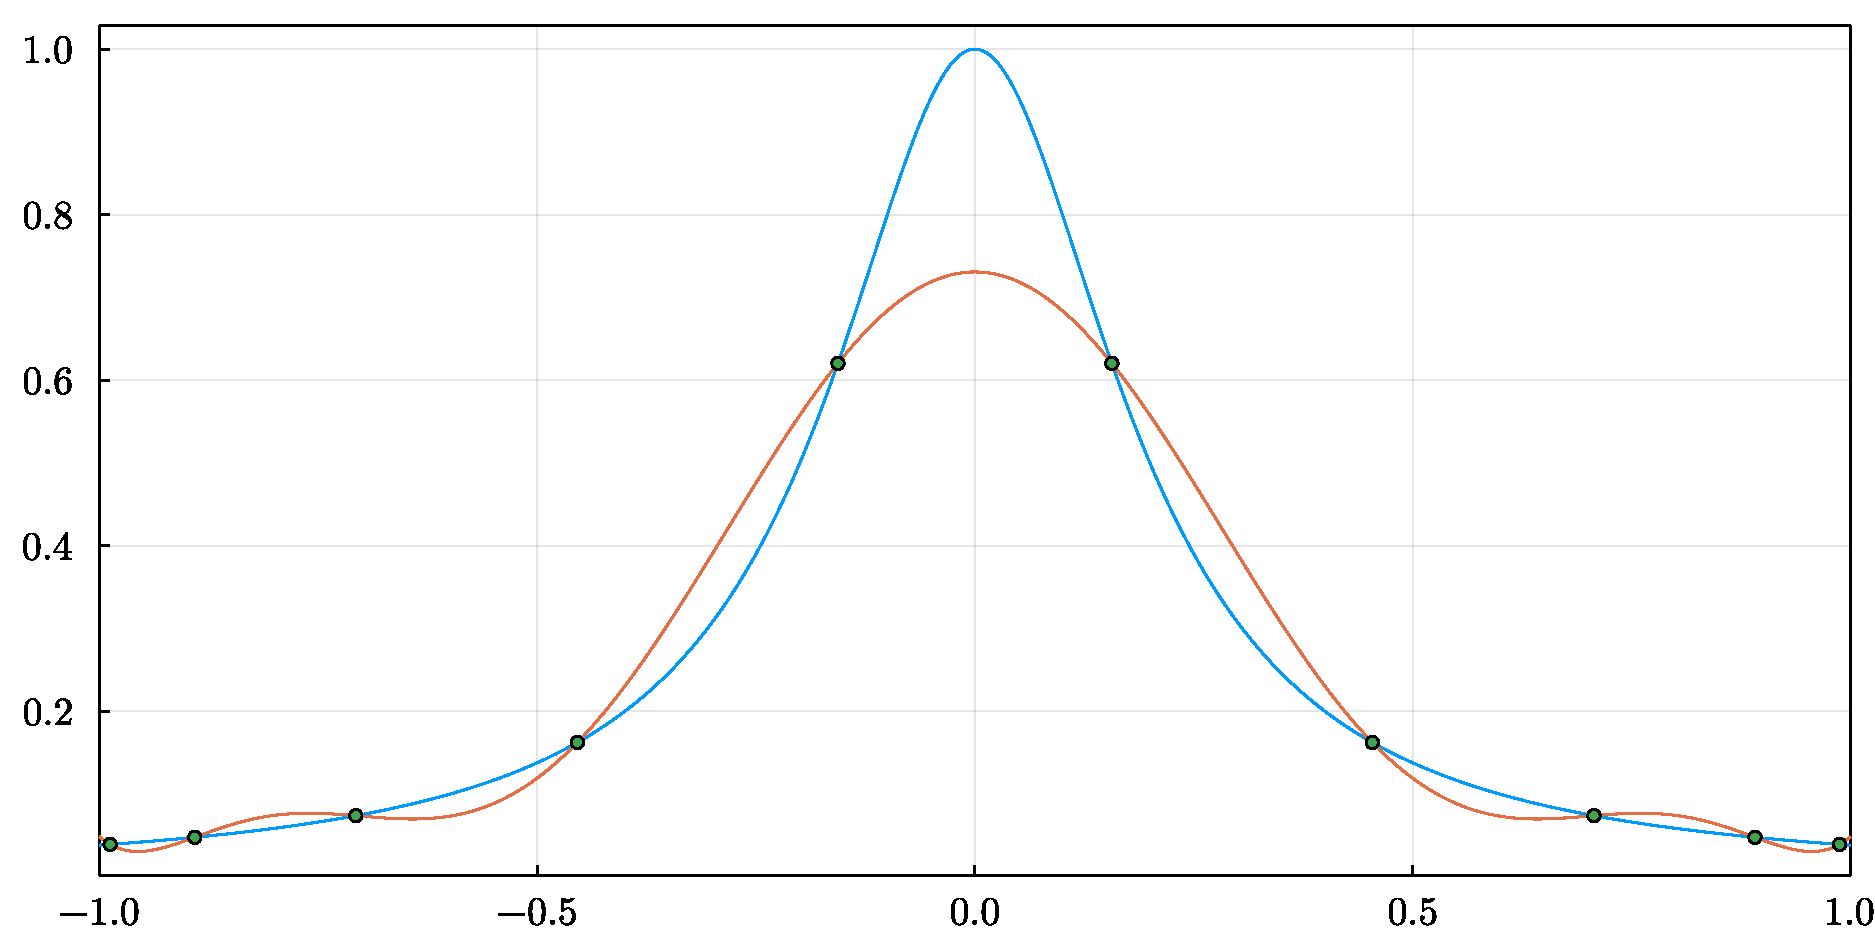
\includegraphics[width=0.49\linewidth]{figures/interpolation_cheb_runge_10.pdf}
    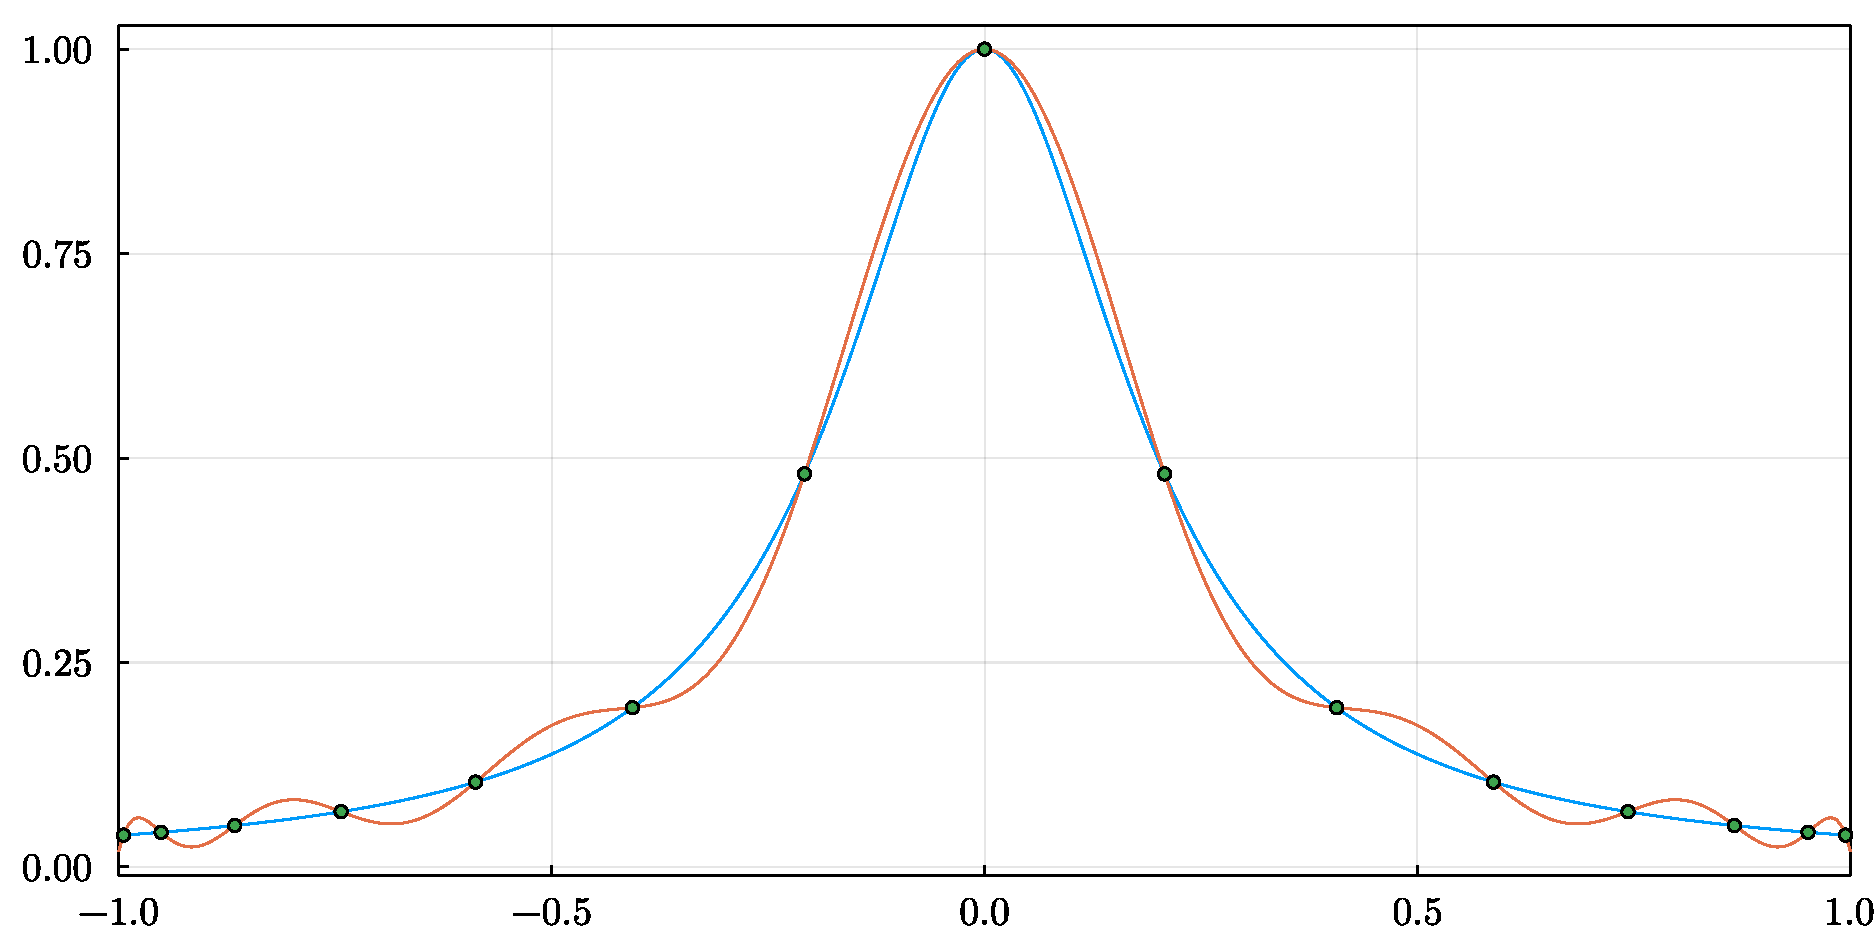
\includegraphics[width=0.49\linewidth]{figures/interpolation_cheb_runge_15.pdf}
    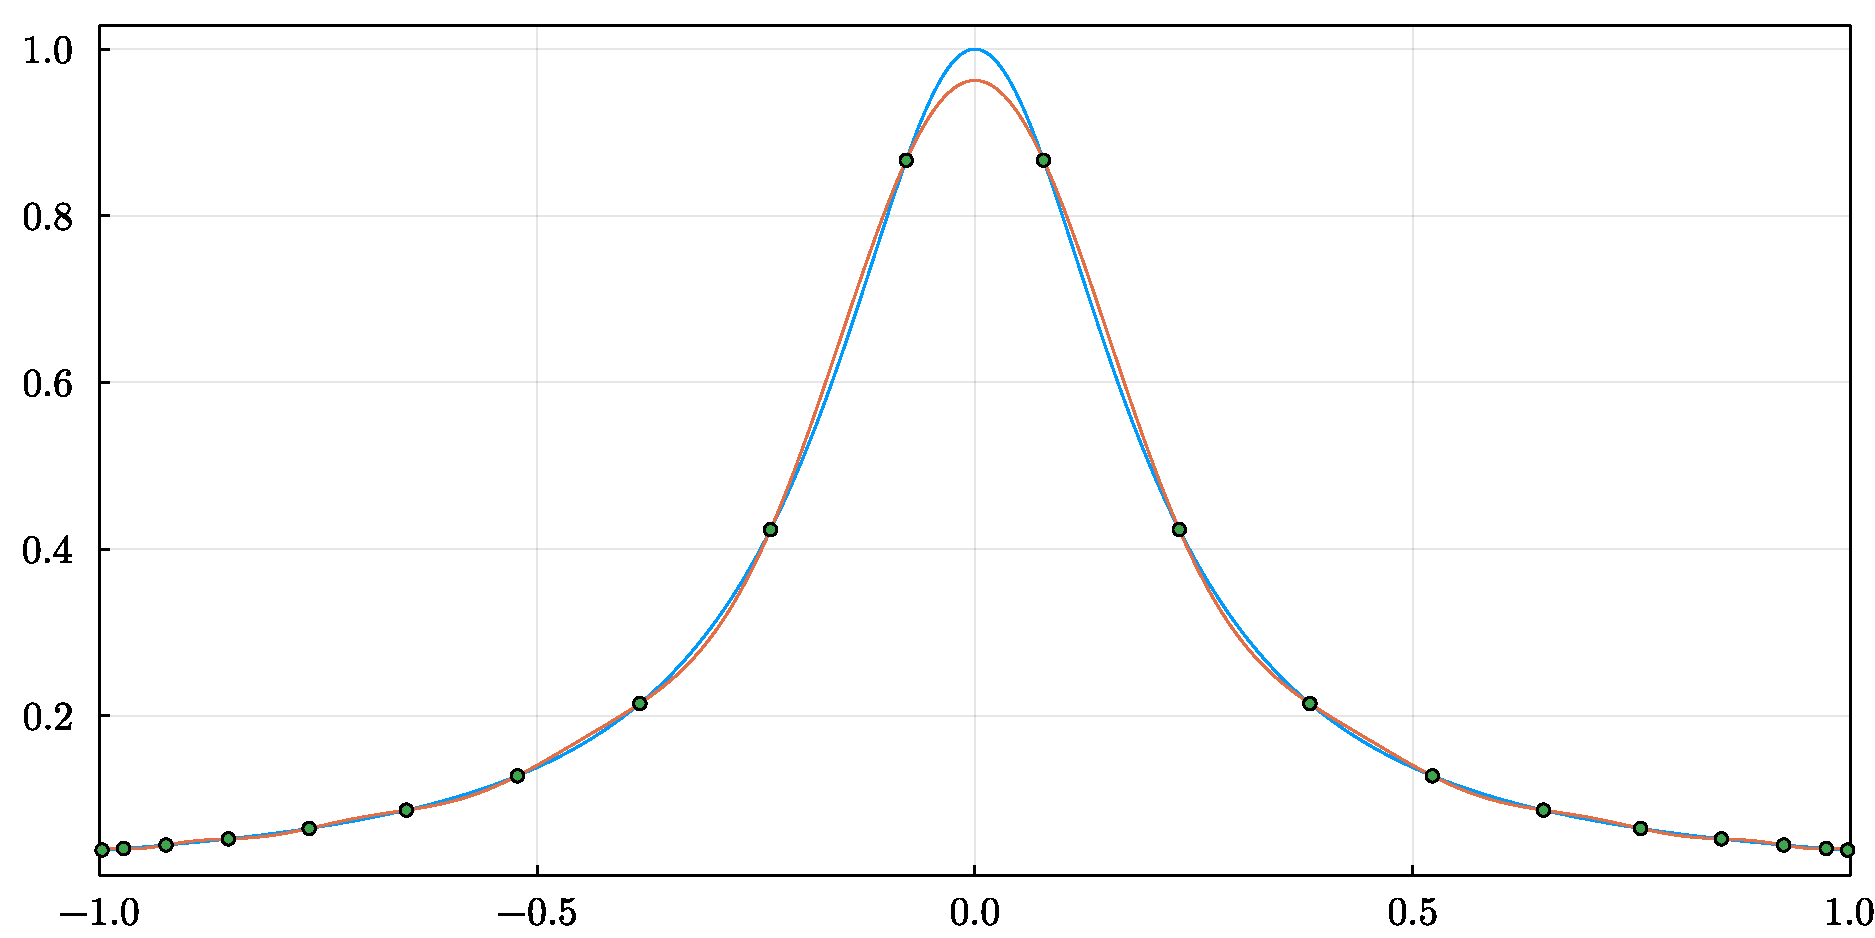
\includegraphics[width=0.49\linewidth]{figures/interpolation_cheb_runge_20.pdf}
    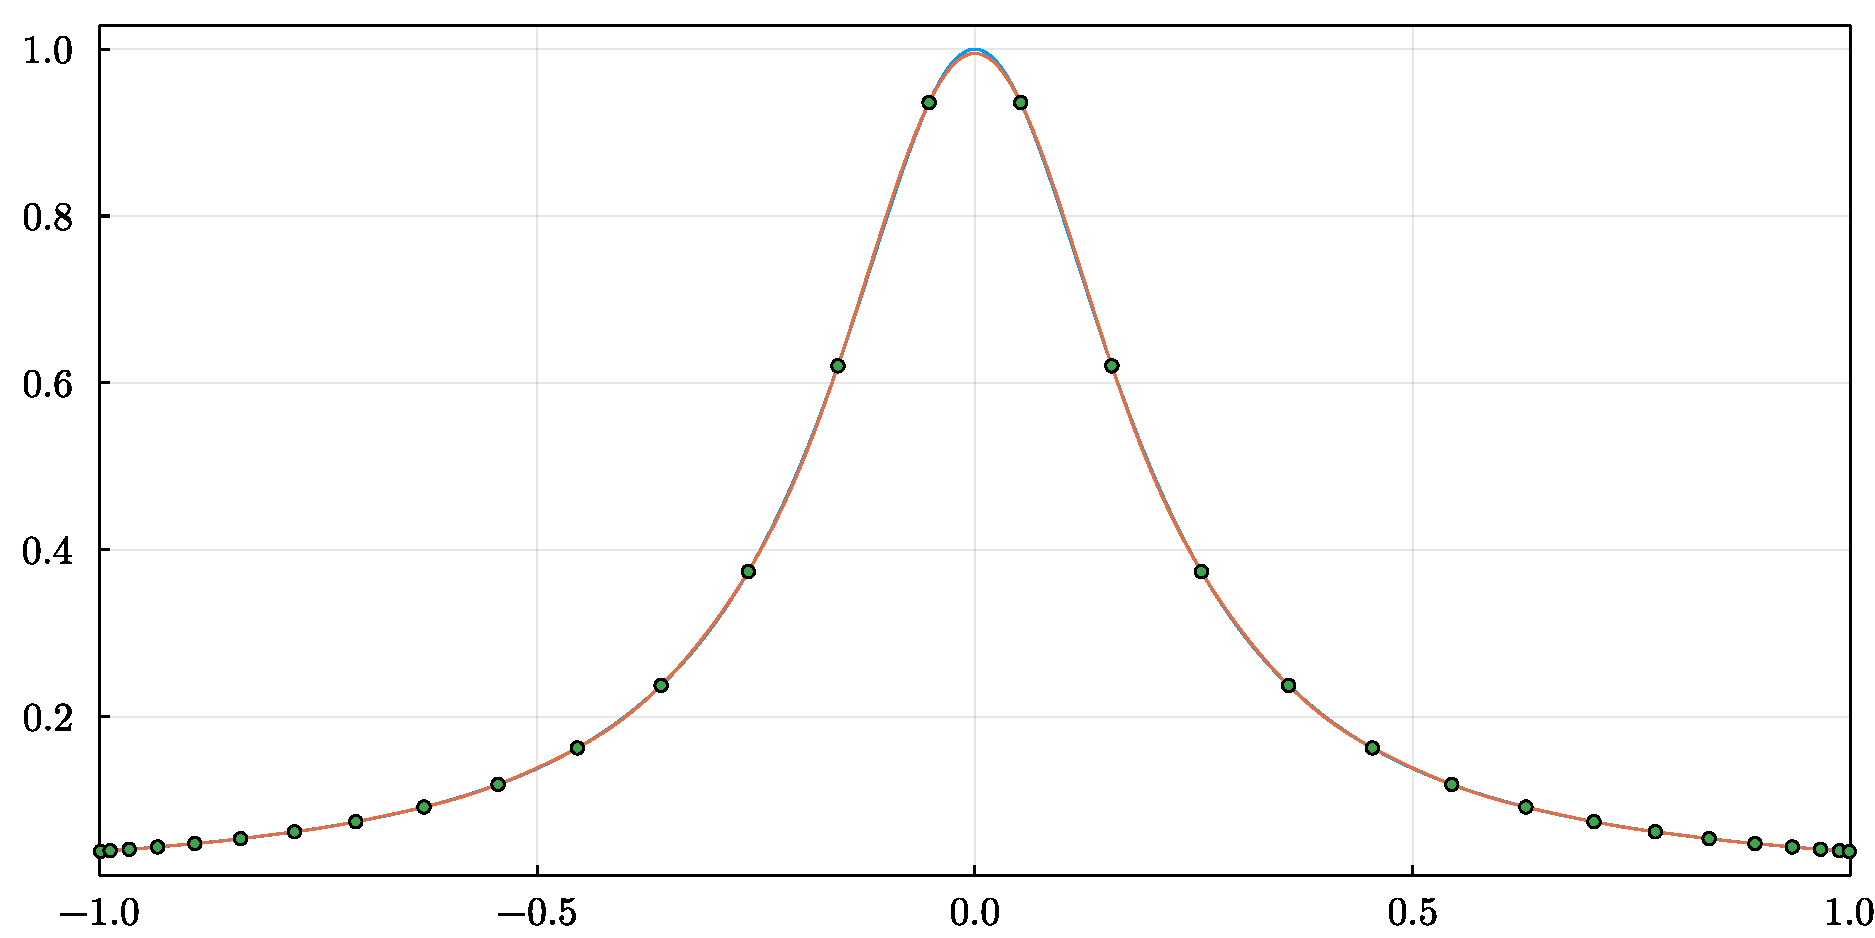
\includegraphics[width=0.49\linewidth]{figures/interpolation_cheb_runge_30.pdf}
    \label{fig:cheb_runge}
\end{figure}

\section{Function approximation}

\begin{exercise}
    Find the polynomial $p(x) = ax + b$ (a straight line) that goes through the points $(x_0, u_0)$ and $(x_1, u_1)$.
\end{exercise}

\begin{exercise}
    Find the polynomial $p(x) = ax^2 + b x + c$ (a parabola) that goes through the points $(0, 1)$, $(1, 3)$ and $(2, 7)$.
\end{exercise}

\begin{exercise}
    Prove the following recurrence relation for Chebyshev polynomials:
    \[
        T_{i+1}(x) = 2 x T_i(x) - T_{i-1}(x), \qquad i = 1, 2, \dotsc.
    \]
\end{exercise}

\begin{exercise}
    \label{exercise:divided_differences}
    Show by recursion that
    \[
        [u_{0}, u_{1}, \dotsc, u_{n}] = \sum_{j=0}^{n} \frac{u_{j}}{\prod_{ k \in \{0, \dotsc, n\} \backslash \{ j\}} (x_{j} - x_{k})}.
    \]
    Deduce from this identity that
    \[
        [u_{0}, u_{1}, \dotsc, u_{n}] = [u_{\sigma_1}, u_{\sigma_2}, \dotsc, u_{\sigma_n}],
    \]
    for any permutation~$\vect \sigma$ of~$(0, 1, 2, \dotsc, n)$.
\end{exercise}

\begin{exercise}
    Using the Gregory--Newton formula,
    find an expression for
    \[
        \sum_{i=1}^{n} i^4.
    \]
\end{exercise}

\begin{exercise}
    Let $(f_0, f_1, f_2, \dotsc) = (1, 1, 2, \dotsc)$ denote the Fibonacci sequence.
    Prove that there does not exist a polynomial~$p$ such that
    \[
        \forall i \in \nat, \qquad
        f_i = p(i).
    \]
\end{exercise}

\begin{exercise}
    Using the Gregory--Newton formula,
    show that
    \begin{equation}
        \label{eq:discrete_exponential}
        \forall n \in \nat_{>0},
        \qquad 2^n = 1 + n + \frac{n^{\underline{2}}}{2!} + \frac{n^{\underline 3}}{3!} + \frac{n^{\underline 4}}{4!} + \dotsb
    \end{equation}
    \begin{remark}
        Remarkably, equation~\eqref{eq:discrete_exponential} holds in fact for \emph{any} $n \in \real_{> 0}$.
        However, showing this more general statement is beyond the scope of this course.
    \end{remark}
\end{exercise}

\begin{compexercise}
    Write a Julia code for interpolating the following function using a polynomial of degree 20.
    \[
        f(x) = \tanh\left(\frac{x+1/2}{\varepsilon}\right) + \tanh\left(\frac{x}{\varepsilon}\right) + \tanh\left(\frac{x-1/2}{\varepsilon}\right),
        \qquad \varepsilon = .01.
    \]
    Use equidistant and then Chebyshev nodes,
    and compare the two approaches in terms of accuracy.
    Plot the function~$f$ together with the approximating polynomials.
\end{compexercise}

\begin{compexercise}
    We wish to use interpolation to approximate the following parametric function:
    \begin{align}
      x (\theta) &= (R - r)\cos\theta + d\cos\left({R - r \over r}\theta\right) \\
      y (\theta) &= (R - r)\sin\theta - d\sin\left({R - r \over r}\theta\right),
    \end{align}
    with $R = 3$, $r = 3$ and $d = 5$, and for $\theta \in [0, 6\pi]$.
    Write a Julia program to interpolate $x(\theta)$ and $y(\theta)$ using 30 equidistant points in the interval $[0, 30]$.
    After constructing the polynomial interpolations $\widehat x(\theta)$ and $\widehat y(\theta)$,
    plot the curve $\theta \mapsto \bigl(\widehat x(\theta), \widehat y(\theta)\bigr)$.
\end{compexercise}
